\documentclass{article}
\usepackage[final]{neurips_2025}  % NEURIPS style (neurips_2025.sty is in paper_draft/)
\makeatletter\providecommand{\@trackname}{}\makeatother
\usepackage[hidelinks]{hyperref}  % REQUIRED: clickable links
\usepackage{booktabs}  % REQUIRED: professional tables
\usepackage{graphicx}
\usepackage{amsmath,amssymb}
\usepackage{amsthm}
\usepackage{enumitem}
\usepackage{algorithm}
\usepackage[noend]{algpseudocode}

% Import command files
%%%%% MATH NOTATION MACROS %%%%%
% Standard math notation for academic papers
% Import with: %%%%% MATH NOTATION MACROS %%%%%
% Standard math notation for academic papers
% Import with: %%%%% MATH NOTATION MACROS %%%%%
% Standard math notation for academic papers
% Import with: \input{commands/math}

\usepackage{amsmath,amsfonts,bm}

%%%%%%%%%%%%%%%%%%%%%%%%%%%%%%%%%%%%%%%%%%%%%%%%%%%%%%%%%%%%%%%%%
% FIGURE AND SECTION REFERENCES
%%%%%%%%%%%%%%%%%%%%%%%%%%%%%%%%%%%%%%%%%%%%%%%%%%%%%%%%%%%%%%%%%

% Mark sections of captions for referring to divisions of figures
\newcommand{\figleft}{{\em (Left)}}
\newcommand{\figcenter}{{\em (Center)}}
\newcommand{\figright}{{\em (Right)}}
\newcommand{\figtop}{{\em (Top)}}
\newcommand{\figbottom}{{\em (Bottom)}}
\newcommand{\captiona}{{\em (a)}}
\newcommand{\captionb}{{\em (b)}}
\newcommand{\captionc}{{\em (c)}}
\newcommand{\captiond}{{\em (d)}}

% Figure references
\def\figref#1{figure~\ref{#1}}
\def\Figref#1{Figure~\ref{#1}}
\def\twofigref#1#2{figures \ref{#1} and \ref{#2}}
\def\quadfigref#1#2#3#4{figures \ref{#1}, \ref{#2}, \ref{#3} and \ref{#4}}

% Section references
\def\secref#1{section~\ref{#1}}
\def\Secref#1{Section~\ref{#1}}
\def\twosecrefs#1#2{sections \ref{#1} and \ref{#2}}
\def\secrefs#1#2#3{sections \ref{#1}, \ref{#2} and \ref{#3}}

% Equation references
\def\eqref#1{equation~\ref{#1}}
\def\Eqref#1{Equation~\ref{#1}}
\def\plaineqref#1{\ref{#1}}

% Algorithm references
\def\algref#1{algorithm~\ref{#1}}
\def\Algref#1{Algorithm~\ref{#1}}
\def\twoalgref#1#2{algorithms \ref{#1} and \ref{#2}}
\def\Twoalgref#1#2{Algorithms \ref{#1} and \ref{#2}}

% Table references
\def\tabref#1{table~\ref{#1}}
\def\Tabref#1{Table~\ref{#1}}

% Chapter references
\def\chapref#1{chapter~\ref{#1}}
\def\Chapref#1{Chapter~\ref{#1}}

%%%%%%%%%%%%%%%%%%%%%%%%%%%%%%%%%%%%%%%%%%%%%%%%%%%%%%%%%%%%%%%%%
% BASIC MATH DEFINITIONS
%%%%%%%%%%%%%%%%%%%%%%%%%%%%%%%%%%%%%%%%%%%%%%%%%%%%%%%%%%%%%%%%%

\def\ceil#1{\lceil #1 \rceil}
\def\floor#1{\lfloor #1 \rfloor}
\def\1{\bm{1}}
\def\eps{{\epsilon}}

% Common operators
\DeclareMathOperator*{\argmax}{arg\,max}
\DeclareMathOperator*{\argmin}{arg\,min}
\DeclareMathOperator{\sign}{sign}
\DeclareMathOperator{\Tr}{Tr}
\let\ab\allowbreak

%%%%%%%%%%%%%%%%%%%%%%%%%%%%%%%%%%%%%%%%%%%%%%%%%%%%%%%%%%%%%%%%%
% VECTORS (lowercase bold)
%%%%%%%%%%%%%%%%%%%%%%%%%%%%%%%%%%%%%%%%%%%%%%%%%%%%%%%%%%%%%%%%%

\def\vzero{{\bm{0}}}
\def\vone{{\bm{1}}}
\def\vmu{{\bm{\mu}}}
\def\vtheta{{\bm{\theta}}}
\def\va{{\bm{a}}}
\def\vb{{\bm{b}}}
\def\vc{{\bm{c}}}
\def\vd{{\bm{d}}}
\def\ve{{\bm{e}}}
\def\vf{{\bm{f}}}
\def\vg{{\bm{g}}}
\def\vh{{\bm{h}}}
\def\vi{{\bm{i}}}
\def\vj{{\bm{j}}}
\def\vk{{\bm{k}}}
\def\vl{{\bm{l}}}
\def\vm{{\bm{m}}}
\def\vn{{\bm{n}}}
\def\vo{{\bm{o}}}
\def\vp{{\bm{p}}}
\def\vq{{\bm{q}}}
\def\vr{{\bm{r}}}
\def\vs{{\bm{s}}}
\def\vt{{\bm{t}}}
\def\vu{{\bm{u}}}
\def\vv{{\bm{v}}}
\def\vw{{\bm{w}}}
\def\vx{{\bm{x}}}
\def\vy{{\bm{y}}}
\def\vz{{\bm{z}}}

%%%%%%%%%%%%%%%%%%%%%%%%%%%%%%%%%%%%%%%%%%%%%%%%%%%%%%%%%%%%%%%%%
% MATRICES (uppercase bold)
%%%%%%%%%%%%%%%%%%%%%%%%%%%%%%%%%%%%%%%%%%%%%%%%%%%%%%%%%%%%%%%%%

\def\mA{{\bm{A}}}
\def\mB{{\bm{B}}}
\def\mC{{\bm{C}}}
\def\mD{{\bm{D}}}
\def\mE{{\bm{E}}}
\def\mF{{\bm{F}}}
\def\mG{{\bm{G}}}
\def\mH{{\bm{H}}}
\def\mI{{\bm{I}}}
\def\mJ{{\bm{J}}}
\def\mK{{\bm{K}}}
\def\mL{{\bm{L}}}
\def\mM{{\bm{M}}}
\def\mN{{\bm{N}}}
\def\mO{{\bm{O}}}
\def\mP{{\bm{P}}}
\def\mQ{{\bm{Q}}}
\def\mR{{\bm{R}}}
\def\mS{{\bm{S}}}
\def\mT{{\bm{T}}}
\def\mU{{\bm{U}}}
\def\mV{{\bm{V}}}
\def\mW{{\bm{W}}}
\def\mX{{\bm{X}}}
\def\mY{{\bm{Y}}}
\def\mZ{{\bm{Z}}}
\def\mBeta{{\bm{\beta}}}
\def\mPhi{{\bm{\Phi}}}
\def\mLambda{{\bm{\Lambda}}}
\def\mSigma{{\bm{\Sigma}}}

%%%%%%%%%%%%%%%%%%%%%%%%%%%%%%%%%%%%%%%%%%%%%%%%%%%%%%%%%%%%%%%%%
% CALLIGRAPHIC (mathcal)
%%%%%%%%%%%%%%%%%%%%%%%%%%%%%%%%%%%%%%%%%%%%%%%%%%%%%%%%%%%%%%%%%

\def\gA{{\mathcal{A}}}
\def\gB{{\mathcal{B}}}
\def\gC{{\mathcal{C}}}
\def\gD{{\mathcal{D}}}
\def\gE{{\mathcal{E}}}
\def\gF{{\mathcal{F}}}
\def\gG{{\mathcal{G}}}
\def\gH{{\mathcal{H}}}
\def\gI{{\mathcal{I}}}
\def\gJ{{\mathcal{J}}}
\def\gK{{\mathcal{K}}}
\def\gL{{\mathcal{L}}}
\def\gM{{\mathcal{M}}}
\def\gN{{\mathcal{N}}}
\def\gO{{\mathcal{O}}}
\def\gP{{\mathcal{P}}}
\def\gQ{{\mathcal{Q}}}
\def\gR{{\mathcal{R}}}
\def\gS{{\mathcal{S}}}
\def\gT{{\mathcal{T}}}
\def\gU{{\mathcal{U}}}
\def\gV{{\mathcal{V}}}
\def\gW{{\mathcal{W}}}
\def\gX{{\mathcal{X}}}
\def\gY{{\mathcal{Y}}}
\def\gZ{{\mathcal{Z}}}

%%%%%%%%%%%%%%%%%%%%%%%%%%%%%%%%%%%%%%%%%%%%%%%%%%%%%%%%%%%%%%%%%
% SETS (blackboard bold)
%%%%%%%%%%%%%%%%%%%%%%%%%%%%%%%%%%%%%%%%%%%%%%%%%%%%%%%%%%%%%%%%%

\def\sA{{\mathbb{A}}}
\def\sB{{\mathbb{B}}}
\def\sC{{\mathbb{C}}}
\def\sD{{\mathbb{D}}}
\def\sF{{\mathbb{F}}}
\def\sG{{\mathbb{G}}}
\def\sH{{\mathbb{H}}}
\def\sI{{\mathbb{I}}}
\def\sJ{{\mathbb{J}}}
\def\sK{{\mathbb{K}}}
\def\sL{{\mathbb{L}}}
\def\sM{{\mathbb{M}}}
\def\sN{{\mathbb{N}}}
\def\sO{{\mathbb{O}}}
\def\sP{{\mathbb{P}}}
\def\sQ{{\mathbb{Q}}}
\def\sR{{\mathbb{R}}}
\def\sS{{\mathbb{S}}}
\def\sT{{\mathbb{T}}}
\def\sU{{\mathbb{U}}}
\def\sV{{\mathbb{V}}}
\def\sW{{\mathbb{W}}}
\def\sX{{\mathbb{X}}}
\def\sY{{\mathbb{Y}}}
\def\sZ{{\mathbb{Z}}}

%%%%%%%%%%%%%%%%%%%%%%%%%%%%%%%%%%%%%%%%%%%%%%%%%%%%%%%%%%%%%%%%%
% COMMON MATH SHORTCUTS
%%%%%%%%%%%%%%%%%%%%%%%%%%%%%%%%%%%%%%%%%%%%%%%%%%%%%%%%%%%%%%%%%

% Expectation and variance
\newcommand{\E}{\mathbb{E}}
\newcommand{\Var}{\mathrm{Var}}
\newcommand{\Cov}{\mathrm{Cov}}
\newcommand{\R}{\mathbb{R}}

% Datasets
\newcommand{\train}{\mathcal{D}}
\newcommand{\valid}{\mathcal{D_{\mathrm{valid}}}}
\newcommand{\test}{\mathcal{D_{\mathrm{test}}}}

% Distributions
\newcommand{\laplace}{\mathrm{Laplace}}
\newcommand{\Uniform}{\mathrm{Unif}}
\newcommand{\Normal}{\mathrm{Normal}}
\newcommand{\Categorical}{\mathrm{Categorical}}

% Common functions
\newcommand{\softmax}{\mathrm{softmax}}
\newcommand{\sigmoid}{\sigma}
\newcommand{\KL}{D_{\mathrm{KL}}}

% Norms
\newcommand{\normlzero}{L^0}
\newcommand{\normlone}{L^1}
\newcommand{\normltwo}{L^2}
\newcommand{\normlp}{L^p}
\newcommand{\normmax}{L^\infty}

%%%%%%%%%%%%%%%%%%%%%%%%%%%%%%%%%%%%%%%%%%%%%%%%%%%%%%%%%%%%%%%%%
% DEFINITIONS AND HIGHLIGHTING
%%%%%%%%%%%%%%%%%%%%%%%%%%%%%%%%%%%%%%%%%%%%%%%%%%%%%%%%%%%%%%%%%

% Highlight a newly defined term
\newcommand{\newterm}[1]{{\bf #1}}
\newcommand{\defn}[1]{\textbf{#1}}
\newcommand{\defeq}{\mathrel{\stackrel{\textnormal{\tiny def}}{=}}}


\usepackage{amsmath,amsfonts,bm}

%%%%%%%%%%%%%%%%%%%%%%%%%%%%%%%%%%%%%%%%%%%%%%%%%%%%%%%%%%%%%%%%%
% FIGURE AND SECTION REFERENCES
%%%%%%%%%%%%%%%%%%%%%%%%%%%%%%%%%%%%%%%%%%%%%%%%%%%%%%%%%%%%%%%%%

% Mark sections of captions for referring to divisions of figures
\newcommand{\figleft}{{\em (Left)}}
\newcommand{\figcenter}{{\em (Center)}}
\newcommand{\figright}{{\em (Right)}}
\newcommand{\figtop}{{\em (Top)}}
\newcommand{\figbottom}{{\em (Bottom)}}
\newcommand{\captiona}{{\em (a)}}
\newcommand{\captionb}{{\em (b)}}
\newcommand{\captionc}{{\em (c)}}
\newcommand{\captiond}{{\em (d)}}

% Figure references
\def\figref#1{figure~\ref{#1}}
\def\Figref#1{Figure~\ref{#1}}
\def\twofigref#1#2{figures \ref{#1} and \ref{#2}}
\def\quadfigref#1#2#3#4{figures \ref{#1}, \ref{#2}, \ref{#3} and \ref{#4}}

% Section references
\def\secref#1{section~\ref{#1}}
\def\Secref#1{Section~\ref{#1}}
\def\twosecrefs#1#2{sections \ref{#1} and \ref{#2}}
\def\secrefs#1#2#3{sections \ref{#1}, \ref{#2} and \ref{#3}}

% Equation references
\def\eqref#1{equation~\ref{#1}}
\def\Eqref#1{Equation~\ref{#1}}
\def\plaineqref#1{\ref{#1}}

% Algorithm references
\def\algref#1{algorithm~\ref{#1}}
\def\Algref#1{Algorithm~\ref{#1}}
\def\twoalgref#1#2{algorithms \ref{#1} and \ref{#2}}
\def\Twoalgref#1#2{Algorithms \ref{#1} and \ref{#2}}

% Table references
\def\tabref#1{table~\ref{#1}}
\def\Tabref#1{Table~\ref{#1}}

% Chapter references
\def\chapref#1{chapter~\ref{#1}}
\def\Chapref#1{Chapter~\ref{#1}}

%%%%%%%%%%%%%%%%%%%%%%%%%%%%%%%%%%%%%%%%%%%%%%%%%%%%%%%%%%%%%%%%%
% BASIC MATH DEFINITIONS
%%%%%%%%%%%%%%%%%%%%%%%%%%%%%%%%%%%%%%%%%%%%%%%%%%%%%%%%%%%%%%%%%

\def\ceil#1{\lceil #1 \rceil}
\def\floor#1{\lfloor #1 \rfloor}
\def\1{\bm{1}}
\def\eps{{\epsilon}}

% Common operators
\DeclareMathOperator*{\argmax}{arg\,max}
\DeclareMathOperator*{\argmin}{arg\,min}
\DeclareMathOperator{\sign}{sign}
\DeclareMathOperator{\Tr}{Tr}
\let\ab\allowbreak

%%%%%%%%%%%%%%%%%%%%%%%%%%%%%%%%%%%%%%%%%%%%%%%%%%%%%%%%%%%%%%%%%
% VECTORS (lowercase bold)
%%%%%%%%%%%%%%%%%%%%%%%%%%%%%%%%%%%%%%%%%%%%%%%%%%%%%%%%%%%%%%%%%

\def\vzero{{\bm{0}}}
\def\vone{{\bm{1}}}
\def\vmu{{\bm{\mu}}}
\def\vtheta{{\bm{\theta}}}
\def\va{{\bm{a}}}
\def\vb{{\bm{b}}}
\def\vc{{\bm{c}}}
\def\vd{{\bm{d}}}
\def\ve{{\bm{e}}}
\def\vf{{\bm{f}}}
\def\vg{{\bm{g}}}
\def\vh{{\bm{h}}}
\def\vi{{\bm{i}}}
\def\vj{{\bm{j}}}
\def\vk{{\bm{k}}}
\def\vl{{\bm{l}}}
\def\vm{{\bm{m}}}
\def\vn{{\bm{n}}}
\def\vo{{\bm{o}}}
\def\vp{{\bm{p}}}
\def\vq{{\bm{q}}}
\def\vr{{\bm{r}}}
\def\vs{{\bm{s}}}
\def\vt{{\bm{t}}}
\def\vu{{\bm{u}}}
\def\vv{{\bm{v}}}
\def\vw{{\bm{w}}}
\def\vx{{\bm{x}}}
\def\vy{{\bm{y}}}
\def\vz{{\bm{z}}}

%%%%%%%%%%%%%%%%%%%%%%%%%%%%%%%%%%%%%%%%%%%%%%%%%%%%%%%%%%%%%%%%%
% MATRICES (uppercase bold)
%%%%%%%%%%%%%%%%%%%%%%%%%%%%%%%%%%%%%%%%%%%%%%%%%%%%%%%%%%%%%%%%%

\def\mA{{\bm{A}}}
\def\mB{{\bm{B}}}
\def\mC{{\bm{C}}}
\def\mD{{\bm{D}}}
\def\mE{{\bm{E}}}
\def\mF{{\bm{F}}}
\def\mG{{\bm{G}}}
\def\mH{{\bm{H}}}
\def\mI{{\bm{I}}}
\def\mJ{{\bm{J}}}
\def\mK{{\bm{K}}}
\def\mL{{\bm{L}}}
\def\mM{{\bm{M}}}
\def\mN{{\bm{N}}}
\def\mO{{\bm{O}}}
\def\mP{{\bm{P}}}
\def\mQ{{\bm{Q}}}
\def\mR{{\bm{R}}}
\def\mS{{\bm{S}}}
\def\mT{{\bm{T}}}
\def\mU{{\bm{U}}}
\def\mV{{\bm{V}}}
\def\mW{{\bm{W}}}
\def\mX{{\bm{X}}}
\def\mY{{\bm{Y}}}
\def\mZ{{\bm{Z}}}
\def\mBeta{{\bm{\beta}}}
\def\mPhi{{\bm{\Phi}}}
\def\mLambda{{\bm{\Lambda}}}
\def\mSigma{{\bm{\Sigma}}}

%%%%%%%%%%%%%%%%%%%%%%%%%%%%%%%%%%%%%%%%%%%%%%%%%%%%%%%%%%%%%%%%%
% CALLIGRAPHIC (mathcal)
%%%%%%%%%%%%%%%%%%%%%%%%%%%%%%%%%%%%%%%%%%%%%%%%%%%%%%%%%%%%%%%%%

\def\gA{{\mathcal{A}}}
\def\gB{{\mathcal{B}}}
\def\gC{{\mathcal{C}}}
\def\gD{{\mathcal{D}}}
\def\gE{{\mathcal{E}}}
\def\gF{{\mathcal{F}}}
\def\gG{{\mathcal{G}}}
\def\gH{{\mathcal{H}}}
\def\gI{{\mathcal{I}}}
\def\gJ{{\mathcal{J}}}
\def\gK{{\mathcal{K}}}
\def\gL{{\mathcal{L}}}
\def\gM{{\mathcal{M}}}
\def\gN{{\mathcal{N}}}
\def\gO{{\mathcal{O}}}
\def\gP{{\mathcal{P}}}
\def\gQ{{\mathcal{Q}}}
\def\gR{{\mathcal{R}}}
\def\gS{{\mathcal{S}}}
\def\gT{{\mathcal{T}}}
\def\gU{{\mathcal{U}}}
\def\gV{{\mathcal{V}}}
\def\gW{{\mathcal{W}}}
\def\gX{{\mathcal{X}}}
\def\gY{{\mathcal{Y}}}
\def\gZ{{\mathcal{Z}}}

%%%%%%%%%%%%%%%%%%%%%%%%%%%%%%%%%%%%%%%%%%%%%%%%%%%%%%%%%%%%%%%%%
% SETS (blackboard bold)
%%%%%%%%%%%%%%%%%%%%%%%%%%%%%%%%%%%%%%%%%%%%%%%%%%%%%%%%%%%%%%%%%

\def\sA{{\mathbb{A}}}
\def\sB{{\mathbb{B}}}
\def\sC{{\mathbb{C}}}
\def\sD{{\mathbb{D}}}
\def\sF{{\mathbb{F}}}
\def\sG{{\mathbb{G}}}
\def\sH{{\mathbb{H}}}
\def\sI{{\mathbb{I}}}
\def\sJ{{\mathbb{J}}}
\def\sK{{\mathbb{K}}}
\def\sL{{\mathbb{L}}}
\def\sM{{\mathbb{M}}}
\def\sN{{\mathbb{N}}}
\def\sO{{\mathbb{O}}}
\def\sP{{\mathbb{P}}}
\def\sQ{{\mathbb{Q}}}
\def\sR{{\mathbb{R}}}
\def\sS{{\mathbb{S}}}
\def\sT{{\mathbb{T}}}
\def\sU{{\mathbb{U}}}
\def\sV{{\mathbb{V}}}
\def\sW{{\mathbb{W}}}
\def\sX{{\mathbb{X}}}
\def\sY{{\mathbb{Y}}}
\def\sZ{{\mathbb{Z}}}

%%%%%%%%%%%%%%%%%%%%%%%%%%%%%%%%%%%%%%%%%%%%%%%%%%%%%%%%%%%%%%%%%
% COMMON MATH SHORTCUTS
%%%%%%%%%%%%%%%%%%%%%%%%%%%%%%%%%%%%%%%%%%%%%%%%%%%%%%%%%%%%%%%%%

% Expectation and variance
\newcommand{\E}{\mathbb{E}}
\newcommand{\Var}{\mathrm{Var}}
\newcommand{\Cov}{\mathrm{Cov}}
\newcommand{\R}{\mathbb{R}}

% Datasets
\newcommand{\train}{\mathcal{D}}
\newcommand{\valid}{\mathcal{D_{\mathrm{valid}}}}
\newcommand{\test}{\mathcal{D_{\mathrm{test}}}}

% Distributions
\newcommand{\laplace}{\mathrm{Laplace}}
\newcommand{\Uniform}{\mathrm{Unif}}
\newcommand{\Normal}{\mathrm{Normal}}
\newcommand{\Categorical}{\mathrm{Categorical}}

% Common functions
\newcommand{\softmax}{\mathrm{softmax}}
\newcommand{\sigmoid}{\sigma}
\newcommand{\KL}{D_{\mathrm{KL}}}

% Norms
\newcommand{\normlzero}{L^0}
\newcommand{\normlone}{L^1}
\newcommand{\normltwo}{L^2}
\newcommand{\normlp}{L^p}
\newcommand{\normmax}{L^\infty}

%%%%%%%%%%%%%%%%%%%%%%%%%%%%%%%%%%%%%%%%%%%%%%%%%%%%%%%%%%%%%%%%%
% DEFINITIONS AND HIGHLIGHTING
%%%%%%%%%%%%%%%%%%%%%%%%%%%%%%%%%%%%%%%%%%%%%%%%%%%%%%%%%%%%%%%%%

% Highlight a newly defined term
\newcommand{\newterm}[1]{{\bf #1}}
\newcommand{\defn}[1]{\textbf{#1}}
\newcommand{\defeq}{\mathrel{\stackrel{\textnormal{\tiny def}}{=}}}


\usepackage{amsmath,amsfonts,bm}

%%%%%%%%%%%%%%%%%%%%%%%%%%%%%%%%%%%%%%%%%%%%%%%%%%%%%%%%%%%%%%%%%
% FIGURE AND SECTION REFERENCES
%%%%%%%%%%%%%%%%%%%%%%%%%%%%%%%%%%%%%%%%%%%%%%%%%%%%%%%%%%%%%%%%%

% Mark sections of captions for referring to divisions of figures
\newcommand{\figleft}{{\em (Left)}}
\newcommand{\figcenter}{{\em (Center)}}
\newcommand{\figright}{{\em (Right)}}
\newcommand{\figtop}{{\em (Top)}}
\newcommand{\figbottom}{{\em (Bottom)}}
\newcommand{\captiona}{{\em (a)}}
\newcommand{\captionb}{{\em (b)}}
\newcommand{\captionc}{{\em (c)}}
\newcommand{\captiond}{{\em (d)}}

% Figure references
\def\figref#1{figure~\ref{#1}}
\def\Figref#1{Figure~\ref{#1}}
\def\twofigref#1#2{figures \ref{#1} and \ref{#2}}
\def\quadfigref#1#2#3#4{figures \ref{#1}, \ref{#2}, \ref{#3} and \ref{#4}}

% Section references
\def\secref#1{section~\ref{#1}}
\def\Secref#1{Section~\ref{#1}}
\def\twosecrefs#1#2{sections \ref{#1} and \ref{#2}}
\def\secrefs#1#2#3{sections \ref{#1}, \ref{#2} and \ref{#3}}

% Equation references
\def\eqref#1{equation~\ref{#1}}
\def\Eqref#1{Equation~\ref{#1}}
\def\plaineqref#1{\ref{#1}}

% Algorithm references
\def\algref#1{algorithm~\ref{#1}}
\def\Algref#1{Algorithm~\ref{#1}}
\def\twoalgref#1#2{algorithms \ref{#1} and \ref{#2}}
\def\Twoalgref#1#2{Algorithms \ref{#1} and \ref{#2}}

% Table references
\def\tabref#1{table~\ref{#1}}
\def\Tabref#1{Table~\ref{#1}}

% Chapter references
\def\chapref#1{chapter~\ref{#1}}
\def\Chapref#1{Chapter~\ref{#1}}

%%%%%%%%%%%%%%%%%%%%%%%%%%%%%%%%%%%%%%%%%%%%%%%%%%%%%%%%%%%%%%%%%
% BASIC MATH DEFINITIONS
%%%%%%%%%%%%%%%%%%%%%%%%%%%%%%%%%%%%%%%%%%%%%%%%%%%%%%%%%%%%%%%%%

\def\ceil#1{\lceil #1 \rceil}
\def\floor#1{\lfloor #1 \rfloor}
\def\1{\bm{1}}
\def\eps{{\epsilon}}

% Common operators
\DeclareMathOperator*{\argmax}{arg\,max}
\DeclareMathOperator*{\argmin}{arg\,min}
\DeclareMathOperator{\sign}{sign}
\DeclareMathOperator{\Tr}{Tr}
\let\ab\allowbreak

%%%%%%%%%%%%%%%%%%%%%%%%%%%%%%%%%%%%%%%%%%%%%%%%%%%%%%%%%%%%%%%%%
% VECTORS (lowercase bold)
%%%%%%%%%%%%%%%%%%%%%%%%%%%%%%%%%%%%%%%%%%%%%%%%%%%%%%%%%%%%%%%%%

\def\vzero{{\bm{0}}}
\def\vone{{\bm{1}}}
\def\vmu{{\bm{\mu}}}
\def\vtheta{{\bm{\theta}}}
\def\va{{\bm{a}}}
\def\vb{{\bm{b}}}
\def\vc{{\bm{c}}}
\def\vd{{\bm{d}}}
\def\ve{{\bm{e}}}
\def\vf{{\bm{f}}}
\def\vg{{\bm{g}}}
\def\vh{{\bm{h}}}
\def\vi{{\bm{i}}}
\def\vj{{\bm{j}}}
\def\vk{{\bm{k}}}
\def\vl{{\bm{l}}}
\def\vm{{\bm{m}}}
\def\vn{{\bm{n}}}
\def\vo{{\bm{o}}}
\def\vp{{\bm{p}}}
\def\vq{{\bm{q}}}
\def\vr{{\bm{r}}}
\def\vs{{\bm{s}}}
\def\vt{{\bm{t}}}
\def\vu{{\bm{u}}}
\def\vv{{\bm{v}}}
\def\vw{{\bm{w}}}
\def\vx{{\bm{x}}}
\def\vy{{\bm{y}}}
\def\vz{{\bm{z}}}

%%%%%%%%%%%%%%%%%%%%%%%%%%%%%%%%%%%%%%%%%%%%%%%%%%%%%%%%%%%%%%%%%
% MATRICES (uppercase bold)
%%%%%%%%%%%%%%%%%%%%%%%%%%%%%%%%%%%%%%%%%%%%%%%%%%%%%%%%%%%%%%%%%

\def\mA{{\bm{A}}}
\def\mB{{\bm{B}}}
\def\mC{{\bm{C}}}
\def\mD{{\bm{D}}}
\def\mE{{\bm{E}}}
\def\mF{{\bm{F}}}
\def\mG{{\bm{G}}}
\def\mH{{\bm{H}}}
\def\mI{{\bm{I}}}
\def\mJ{{\bm{J}}}
\def\mK{{\bm{K}}}
\def\mL{{\bm{L}}}
\def\mM{{\bm{M}}}
\def\mN{{\bm{N}}}
\def\mO{{\bm{O}}}
\def\mP{{\bm{P}}}
\def\mQ{{\bm{Q}}}
\def\mR{{\bm{R}}}
\def\mS{{\bm{S}}}
\def\mT{{\bm{T}}}
\def\mU{{\bm{U}}}
\def\mV{{\bm{V}}}
\def\mW{{\bm{W}}}
\def\mX{{\bm{X}}}
\def\mY{{\bm{Y}}}
\def\mZ{{\bm{Z}}}
\def\mBeta{{\bm{\beta}}}
\def\mPhi{{\bm{\Phi}}}
\def\mLambda{{\bm{\Lambda}}}
\def\mSigma{{\bm{\Sigma}}}

%%%%%%%%%%%%%%%%%%%%%%%%%%%%%%%%%%%%%%%%%%%%%%%%%%%%%%%%%%%%%%%%%
% CALLIGRAPHIC (mathcal)
%%%%%%%%%%%%%%%%%%%%%%%%%%%%%%%%%%%%%%%%%%%%%%%%%%%%%%%%%%%%%%%%%

\def\gA{{\mathcal{A}}}
\def\gB{{\mathcal{B}}}
\def\gC{{\mathcal{C}}}
\def\gD{{\mathcal{D}}}
\def\gE{{\mathcal{E}}}
\def\gF{{\mathcal{F}}}
\def\gG{{\mathcal{G}}}
\def\gH{{\mathcal{H}}}
\def\gI{{\mathcal{I}}}
\def\gJ{{\mathcal{J}}}
\def\gK{{\mathcal{K}}}
\def\gL{{\mathcal{L}}}
\def\gM{{\mathcal{M}}}
\def\gN{{\mathcal{N}}}
\def\gO{{\mathcal{O}}}
\def\gP{{\mathcal{P}}}
\def\gQ{{\mathcal{Q}}}
\def\gR{{\mathcal{R}}}
\def\gS{{\mathcal{S}}}
\def\gT{{\mathcal{T}}}
\def\gU{{\mathcal{U}}}
\def\gV{{\mathcal{V}}}
\def\gW{{\mathcal{W}}}
\def\gX{{\mathcal{X}}}
\def\gY{{\mathcal{Y}}}
\def\gZ{{\mathcal{Z}}}

%%%%%%%%%%%%%%%%%%%%%%%%%%%%%%%%%%%%%%%%%%%%%%%%%%%%%%%%%%%%%%%%%
% SETS (blackboard bold)
%%%%%%%%%%%%%%%%%%%%%%%%%%%%%%%%%%%%%%%%%%%%%%%%%%%%%%%%%%%%%%%%%

\def\sA{{\mathbb{A}}}
\def\sB{{\mathbb{B}}}
\def\sC{{\mathbb{C}}}
\def\sD{{\mathbb{D}}}
\def\sF{{\mathbb{F}}}
\def\sG{{\mathbb{G}}}
\def\sH{{\mathbb{H}}}
\def\sI{{\mathbb{I}}}
\def\sJ{{\mathbb{J}}}
\def\sK{{\mathbb{K}}}
\def\sL{{\mathbb{L}}}
\def\sM{{\mathbb{M}}}
\def\sN{{\mathbb{N}}}
\def\sO{{\mathbb{O}}}
\def\sP{{\mathbb{P}}}
\def\sQ{{\mathbb{Q}}}
\def\sR{{\mathbb{R}}}
\def\sS{{\mathbb{S}}}
\def\sT{{\mathbb{T}}}
\def\sU{{\mathbb{U}}}
\def\sV{{\mathbb{V}}}
\def\sW{{\mathbb{W}}}
\def\sX{{\mathbb{X}}}
\def\sY{{\mathbb{Y}}}
\def\sZ{{\mathbb{Z}}}

%%%%%%%%%%%%%%%%%%%%%%%%%%%%%%%%%%%%%%%%%%%%%%%%%%%%%%%%%%%%%%%%%
% COMMON MATH SHORTCUTS
%%%%%%%%%%%%%%%%%%%%%%%%%%%%%%%%%%%%%%%%%%%%%%%%%%%%%%%%%%%%%%%%%

% Expectation and variance
\newcommand{\E}{\mathbb{E}}
\newcommand{\Var}{\mathrm{Var}}
\newcommand{\Cov}{\mathrm{Cov}}
\newcommand{\R}{\mathbb{R}}

% Datasets
\newcommand{\train}{\mathcal{D}}
\newcommand{\valid}{\mathcal{D_{\mathrm{valid}}}}
\newcommand{\test}{\mathcal{D_{\mathrm{test}}}}

% Distributions
\newcommand{\laplace}{\mathrm{Laplace}}
\newcommand{\Uniform}{\mathrm{Unif}}
\newcommand{\Normal}{\mathrm{Normal}}
\newcommand{\Categorical}{\mathrm{Categorical}}

% Common functions
\newcommand{\softmax}{\mathrm{softmax}}
\newcommand{\sigmoid}{\sigma}
\newcommand{\KL}{D_{\mathrm{KL}}}

% Norms
\newcommand{\normlzero}{L^0}
\newcommand{\normlone}{L^1}
\newcommand{\normltwo}{L^2}
\newcommand{\normlp}{L^p}
\newcommand{\normmax}{L^\infty}

%%%%%%%%%%%%%%%%%%%%%%%%%%%%%%%%%%%%%%%%%%%%%%%%%%%%%%%%%%%%%%%%%
% DEFINITIONS AND HIGHLIGHTING
%%%%%%%%%%%%%%%%%%%%%%%%%%%%%%%%%%%%%%%%%%%%%%%%%%%%%%%%%%%%%%%%%

% Highlight a newly defined term
\newcommand{\newterm}[1]{{\bf #1}}
\newcommand{\defn}[1]{\textbf{#1}}
\newcommand{\defeq}{\mathrel{\stackrel{\textnormal{\tiny def}}{=}}}

%%%%% GENERAL FORMATTING MACROS %%%%%
% General formatting and styling macros for academic papers
% Import with: %%%%% GENERAL FORMATTING MACROS %%%%%
% General formatting and styling macros for academic papers
% Import with: %%%%% GENERAL FORMATTING MACROS %%%%%
% General formatting and styling macros for academic papers
% Import with: \input{commands/general}

%%%%%%%%%%%%%%%%%%%%%%%%%%%%%%%%%%%%%%%%%%%%%%%%%%%%%%%%%%%%%%%%%
% PARAGRAPH AND TEXT FORMATTING
%%%%%%%%%%%%%%%%%%%%%%%%%%%%%%%%%%%%%%%%%%%%%%%%%%%%%%%%%%%%%%%%%

% Bold paragraph headers (use: \para{Header.} followed by text)
\newcommand{\para}[1]{\noindent \textbf{#1}}

% Cut content for space (content is hidden but preserved in source)
\newcommand{\cutforspace}[1]{}

% Response/rebuttal formatting for reviews
\newcommand{\response}[1]{\vspace{3pt}\hrule\vspace{3pt}\textbf{#1:}}

%%%%%%%%%%%%%%%%%%%%%%%%%%%%%%%%%%%%%%%%%%%%%%%%%%%%%%%%%%%%%%%%%
% RESULT HIGHLIGHTING
%%%%%%%%%%%%%%%%%%%%%%%%%%%%%%%%%%%%%%%%%%%%%%%%%%%%%%%%%%%%%%%%%

\usepackage{xcolor}
\usepackage{bm}

% Colors for result arrows
\definecolor{pastelgreen}{RGB}{50,205,50}

% Arrows for showing improvement/decline in results
\newcommand{\increase}{\textcolor{pastelgreen}{\bm{$\uparrow$}}}
\newcommand{\decrease}{\textcolor{red}{\bm{$\downarrow$}}}

% Phantom star for alignment in tables (use where no significance marker needed)
\newcommand{\pstar}{\phantom{*}}

%%%%%%%%%%%%%%%%%%%%%%%%%%%%%%%%%%%%%%%%%%%%%%%%%%%%%%%%%%%%%%%%%
% HIGHLIGHT BOXES
%%%%%%%%%%%%%%%%%%%%%%%%%%%%%%%%%%%%%%%%%%%%%%%%%%%%%%%%%%%%%%%%%

% Background colors for highlight boxes
\definecolor{aigold}{RGB}{244,210,1}
\definecolor{aigreen}{RGB}{213,245,227}
\definecolor{humanpurple}{RGB}{235,222,240}
\definecolor{aired}{RGB}{255,180,181}
\definecolor{mypurple}{RGB}{147,112,219}
\definecolor{myorange}{RGB}{255,165,0}
\definecolor{commentgray}{RGB}{86,101,115}
\definecolor{mygray}{RGB}{169,169,169}

% Highlight boxes for examples, quotes, etc.
\newcommand{\lightgreen}[1]{\fcolorbox{aigreen}{aigreen}{\parbox{\linewidth}{#1}}}
\newcommand{\lightred}[1]{\colorbox{aired}{\parbox{\linewidth}{#1}}}

%%%%%%%%%%%%%%%%%%%%%%%%%%%%%%%%%%%%%%%%%%%%%%%%%%%%%%%%%%%%%%%%%
% ALGORITHM STYLING
%%%%%%%%%%%%%%%%%%%%%%%%%%%%%%%%%%%%%%%%%%%%%%%%%%%%%%%%%%%%%%%%%

% Comment style for algorithms (triangleright marker)
\newcommand{\rightcomment}[1]{\(\triangleright\) {\small \it #1}}

% Equation comments
\newcommand{\eqcomment}[1]{\addtocounter{equation}{1}\tag*{\rightcomment{#1}\quad(\theequation)}}

% Algorithm formatting (requires algorithm and algpseudocode packages)
% \usepackage{algorithm}
% \usepackage[noend]{algpseudocode}

% Customize algorithm appearance
\renewcommand{\algorithmicindent}{9pt}
% \renewcommand\algorithmicdo{:}
% \renewcommand\algorithmicthen{:}

% Algorithm input/output
% \algnewcommand\algorithmicinput{{\bfseries Input:}}
% \algnewcommand\INPUT{\item[\algorithmicinput]}
% \algnewcommand\algorithmicoutput{{\bfseries Output:}}
% \algnewcommand\OUTPUT{\item[\algorithmicoutput]}

%%%%%%%%%%%%%%%%%%%%%%%%%%%%%%%%%%%%%%%%%%%%%%%%%%%%%%%%%%%%%%%%%
% CODE LISTINGS
%%%%%%%%%%%%%%%%%%%%%%%%%%%%%%%%%%%%%%%%%%%%%%%%%%%%%%%%%%%%%%%%%

\usepackage{listings}

\definecolor{codepurple}{RGB}{128,0,128}

\lstdefinestyle{datalogstyle}{
    basicstyle={\tt \scriptsize},
    xleftmargin={6pt},
    xrightmargin={6pt},
    columns=flexible,
    breakindent=0pt,
    breaklines=true,
    frame=tb,
    stepnumber=1,
    firstnumber=1,
    numberfirstline=true,
    tabsize=2,
    extendedchars=true,
    columns=fullflexible,
    keepspaces=true,
    escapeinside={@}{@},
    captionpos=b,
    commentstyle=\color{black!65},
    numberstyle=\tiny\color{black!65},
    stringstyle=\color{codepurple},
    breakatwhitespace=false,
    mathescape=true,
    numbersep=5pt,
    showspaces=false,
    showstringspaces=false,
    showtabs=false,
    aboveskip={0.8\baselineskip},
    belowskip={0.2\baselineskip},
}
\lstset{style=datalogstyle}

% Rename listings to "Example"
\renewcommand{\lstlistingname}{Example}

% Vertical dots for code continuation
\newcommand{\progvdots}{\\[-4pt]$\vdots$}

%%%%%%%%%%%%%%%%%%%%%%%%%%%%%%%%%%%%%%%%%%%%%%%%%%%%%%%%%%%%%%%%%
% AUTHOR COMMENT SYSTEM
%%%%%%%%%%%%%%%%%%%%%%%%%%%%%%%%%%%%%%%%%%%%%%%%%%%%%%%%%%%%%%%%%

% Toggle to hide/show comments (uncomment \hidecommentstrue to hide)
\newif\ifhidecomments
% \hidecommentstrue

% Define author comments (add your own authors here)
% Each author gets a unique color
\ifhidecomments
    % Hidden mode - comments are invisible
    \newcommand{\authorone}[1]{}
    \newcommand{\authortwo}[1]{}
    \newcommand{\authorthree}[1]{}
\else
    % Visible mode - comments shown in color
    \newcommand{\authorone}[1]{\textcolor{blue}{[\textsc{AuthorOne}: #1]}}
    \newcommand{\authortwo}[1]{\textcolor{green!70!blue}{[\textsc{AuthorTwo}: #1]}}
    \newcommand{\authorthree}[1]{\textcolor{magenta!80!brown}{[\textsc{AuthorThree}: #1]}}
\fi

% Generic fixme/todo command
\newcommand{\fixme}[1]{\textcolor{red}{[FIXME: #1]}}

%%%%%%%%%%%%%%%%%%%%%%%%%%%%%%%%%%%%%%%%%%%%%%%%%%%%%%%%%%%%%%%%%
% SPACING CONFIGURATION
%%%%%%%%%%%%%%%%%%%%%%%%%%%%%%%%%%%%%%%%%%%%%%%%%%%%%%%%%%%%%%%%%

% Tight spacing for figures and tables (adjust as needed)
% \captionsetup[subfigure]{aboveskip=2pt,belowskip=2pt}
% \captionsetup[table]{aboveskip=4pt,belowskip=4pt}
% \captionsetup[figure]{aboveskip=4pt,belowskip=4pt}
% \setlength{\dbltextfloatsep}{11pt}
% \setlength{\dblfloatsep}{11pt}
% \setlength{\floatsep}{11pt}
% \setlength{\textfloatsep}{11pt}

%%%%%%%%%%%%%%%%%%%%%%%%%%%%%%%%%%%%%%%%%%%%%%%%%%%%%%%%%%%%%%%%%
% MISCELLANEOUS
%%%%%%%%%%%%%%%%%%%%%%%%%%%%%%%%%%%%%%%%%%%%%%%%%%%%%%%%%%%%%%%%%

% Ordinals
\renewcommand{\th}{\textsuperscript{th}\xspace}

% Special tokens
\newcommand{\bos}{\textsc{bos}\xspace}
\newcommand{\eos}{\textsc{eos}\xspace}

% Inverse notation
\newcommand{\inv}[1]{#1^{\scriptscriptstyle-\!1}}


%%%%%%%%%%%%%%%%%%%%%%%%%%%%%%%%%%%%%%%%%%%%%%%%%%%%%%%%%%%%%%%%%
% PARAGRAPH AND TEXT FORMATTING
%%%%%%%%%%%%%%%%%%%%%%%%%%%%%%%%%%%%%%%%%%%%%%%%%%%%%%%%%%%%%%%%%

% Bold paragraph headers (use: \para{Header.} followed by text)
\newcommand{\para}[1]{\noindent \textbf{#1}}

% Cut content for space (content is hidden but preserved in source)
\newcommand{\cutforspace}[1]{}

% Response/rebuttal formatting for reviews
\newcommand{\response}[1]{\vspace{3pt}\hrule\vspace{3pt}\textbf{#1:}}

%%%%%%%%%%%%%%%%%%%%%%%%%%%%%%%%%%%%%%%%%%%%%%%%%%%%%%%%%%%%%%%%%
% RESULT HIGHLIGHTING
%%%%%%%%%%%%%%%%%%%%%%%%%%%%%%%%%%%%%%%%%%%%%%%%%%%%%%%%%%%%%%%%%

\usepackage{xcolor}
\usepackage{bm}

% Colors for result arrows
\definecolor{pastelgreen}{RGB}{50,205,50}

% Arrows for showing improvement/decline in results
\newcommand{\increase}{\textcolor{pastelgreen}{\bm{$\uparrow$}}}
\newcommand{\decrease}{\textcolor{red}{\bm{$\downarrow$}}}

% Phantom star for alignment in tables (use where no significance marker needed)
\newcommand{\pstar}{\phantom{*}}

%%%%%%%%%%%%%%%%%%%%%%%%%%%%%%%%%%%%%%%%%%%%%%%%%%%%%%%%%%%%%%%%%
% HIGHLIGHT BOXES
%%%%%%%%%%%%%%%%%%%%%%%%%%%%%%%%%%%%%%%%%%%%%%%%%%%%%%%%%%%%%%%%%

% Background colors for highlight boxes
\definecolor{aigold}{RGB}{244,210,1}
\definecolor{aigreen}{RGB}{213,245,227}
\definecolor{humanpurple}{RGB}{235,222,240}
\definecolor{aired}{RGB}{255,180,181}
\definecolor{mypurple}{RGB}{147,112,219}
\definecolor{myorange}{RGB}{255,165,0}
\definecolor{commentgray}{RGB}{86,101,115}
\definecolor{mygray}{RGB}{169,169,169}

% Highlight boxes for examples, quotes, etc.
\newcommand{\lightgreen}[1]{\fcolorbox{aigreen}{aigreen}{\parbox{\linewidth}{#1}}}
\newcommand{\lightred}[1]{\colorbox{aired}{\parbox{\linewidth}{#1}}}

%%%%%%%%%%%%%%%%%%%%%%%%%%%%%%%%%%%%%%%%%%%%%%%%%%%%%%%%%%%%%%%%%
% ALGORITHM STYLING
%%%%%%%%%%%%%%%%%%%%%%%%%%%%%%%%%%%%%%%%%%%%%%%%%%%%%%%%%%%%%%%%%

% Comment style for algorithms (triangleright marker)
\newcommand{\rightcomment}[1]{\(\triangleright\) {\small \it #1}}

% Equation comments
\newcommand{\eqcomment}[1]{\addtocounter{equation}{1}\tag*{\rightcomment{#1}\quad(\theequation)}}

% Algorithm formatting (requires algorithm and algpseudocode packages)
% \usepackage{algorithm}
% \usepackage[noend]{algpseudocode}

% Customize algorithm appearance
\renewcommand{\algorithmicindent}{9pt}
% \renewcommand\algorithmicdo{:}
% \renewcommand\algorithmicthen{:}

% Algorithm input/output
% \algnewcommand\algorithmicinput{{\bfseries Input:}}
% \algnewcommand\INPUT{\item[\algorithmicinput]}
% \algnewcommand\algorithmicoutput{{\bfseries Output:}}
% \algnewcommand\OUTPUT{\item[\algorithmicoutput]}

%%%%%%%%%%%%%%%%%%%%%%%%%%%%%%%%%%%%%%%%%%%%%%%%%%%%%%%%%%%%%%%%%
% CODE LISTINGS
%%%%%%%%%%%%%%%%%%%%%%%%%%%%%%%%%%%%%%%%%%%%%%%%%%%%%%%%%%%%%%%%%

\usepackage{listings}

\definecolor{codepurple}{RGB}{128,0,128}

\lstdefinestyle{datalogstyle}{
    basicstyle={\tt \scriptsize},
    xleftmargin={6pt},
    xrightmargin={6pt},
    columns=flexible,
    breakindent=0pt,
    breaklines=true,
    frame=tb,
    stepnumber=1,
    firstnumber=1,
    numberfirstline=true,
    tabsize=2,
    extendedchars=true,
    columns=fullflexible,
    keepspaces=true,
    escapeinside={@}{@},
    captionpos=b,
    commentstyle=\color{black!65},
    numberstyle=\tiny\color{black!65},
    stringstyle=\color{codepurple},
    breakatwhitespace=false,
    mathescape=true,
    numbersep=5pt,
    showspaces=false,
    showstringspaces=false,
    showtabs=false,
    aboveskip={0.8\baselineskip},
    belowskip={0.2\baselineskip},
}
\lstset{style=datalogstyle}

% Rename listings to "Example"
\renewcommand{\lstlistingname}{Example}

% Vertical dots for code continuation
\newcommand{\progvdots}{\\[-4pt]$\vdots$}

%%%%%%%%%%%%%%%%%%%%%%%%%%%%%%%%%%%%%%%%%%%%%%%%%%%%%%%%%%%%%%%%%
% AUTHOR COMMENT SYSTEM
%%%%%%%%%%%%%%%%%%%%%%%%%%%%%%%%%%%%%%%%%%%%%%%%%%%%%%%%%%%%%%%%%

% Toggle to hide/show comments (uncomment \hidecommentstrue to hide)
\newif\ifhidecomments
% \hidecommentstrue

% Define author comments (add your own authors here)
% Each author gets a unique color
\ifhidecomments
    % Hidden mode - comments are invisible
    \newcommand{\authorone}[1]{}
    \newcommand{\authortwo}[1]{}
    \newcommand{\authorthree}[1]{}
\else
    % Visible mode - comments shown in color
    \newcommand{\authorone}[1]{\textcolor{blue}{[\textsc{AuthorOne}: #1]}}
    \newcommand{\authortwo}[1]{\textcolor{green!70!blue}{[\textsc{AuthorTwo}: #1]}}
    \newcommand{\authorthree}[1]{\textcolor{magenta!80!brown}{[\textsc{AuthorThree}: #1]}}
\fi

% Generic fixme/todo command
\newcommand{\fixme}[1]{\textcolor{red}{[FIXME: #1]}}

%%%%%%%%%%%%%%%%%%%%%%%%%%%%%%%%%%%%%%%%%%%%%%%%%%%%%%%%%%%%%%%%%
% SPACING CONFIGURATION
%%%%%%%%%%%%%%%%%%%%%%%%%%%%%%%%%%%%%%%%%%%%%%%%%%%%%%%%%%%%%%%%%

% Tight spacing for figures and tables (adjust as needed)
% \captionsetup[subfigure]{aboveskip=2pt,belowskip=2pt}
% \captionsetup[table]{aboveskip=4pt,belowskip=4pt}
% \captionsetup[figure]{aboveskip=4pt,belowskip=4pt}
% \setlength{\dbltextfloatsep}{11pt}
% \setlength{\dblfloatsep}{11pt}
% \setlength{\floatsep}{11pt}
% \setlength{\textfloatsep}{11pt}

%%%%%%%%%%%%%%%%%%%%%%%%%%%%%%%%%%%%%%%%%%%%%%%%%%%%%%%%%%%%%%%%%
% MISCELLANEOUS
%%%%%%%%%%%%%%%%%%%%%%%%%%%%%%%%%%%%%%%%%%%%%%%%%%%%%%%%%%%%%%%%%

% Ordinals
\renewcommand{\th}{\textsuperscript{th}\xspace}

% Special tokens
\newcommand{\bos}{\textsc{bos}\xspace}
\newcommand{\eos}{\textsc{eos}\xspace}

% Inverse notation
\newcommand{\inv}[1]{#1^{\scriptscriptstyle-\!1}}


%%%%%%%%%%%%%%%%%%%%%%%%%%%%%%%%%%%%%%%%%%%%%%%%%%%%%%%%%%%%%%%%%
% PARAGRAPH AND TEXT FORMATTING
%%%%%%%%%%%%%%%%%%%%%%%%%%%%%%%%%%%%%%%%%%%%%%%%%%%%%%%%%%%%%%%%%

% Bold paragraph headers (use: \para{Header.} followed by text)
\newcommand{\para}[1]{\noindent \textbf{#1}}

% Cut content for space (content is hidden but preserved in source)
\newcommand{\cutforspace}[1]{}

% Response/rebuttal formatting for reviews
\newcommand{\response}[1]{\vspace{3pt}\hrule\vspace{3pt}\textbf{#1:}}

%%%%%%%%%%%%%%%%%%%%%%%%%%%%%%%%%%%%%%%%%%%%%%%%%%%%%%%%%%%%%%%%%
% RESULT HIGHLIGHTING
%%%%%%%%%%%%%%%%%%%%%%%%%%%%%%%%%%%%%%%%%%%%%%%%%%%%%%%%%%%%%%%%%

\usepackage{xcolor}
\usepackage{bm}

% Colors for result arrows
\definecolor{pastelgreen}{RGB}{50,205,50}

% Arrows for showing improvement/decline in results
\newcommand{\increase}{\textcolor{pastelgreen}{\bm{$\uparrow$}}}
\newcommand{\decrease}{\textcolor{red}{\bm{$\downarrow$}}}

% Phantom star for alignment in tables (use where no significance marker needed)
\newcommand{\pstar}{\phantom{*}}

%%%%%%%%%%%%%%%%%%%%%%%%%%%%%%%%%%%%%%%%%%%%%%%%%%%%%%%%%%%%%%%%%
% HIGHLIGHT BOXES
%%%%%%%%%%%%%%%%%%%%%%%%%%%%%%%%%%%%%%%%%%%%%%%%%%%%%%%%%%%%%%%%%

% Background colors for highlight boxes
\definecolor{aigold}{RGB}{244,210,1}
\definecolor{aigreen}{RGB}{213,245,227}
\definecolor{humanpurple}{RGB}{235,222,240}
\definecolor{aired}{RGB}{255,180,181}
\definecolor{mypurple}{RGB}{147,112,219}
\definecolor{myorange}{RGB}{255,165,0}
\definecolor{commentgray}{RGB}{86,101,115}
\definecolor{mygray}{RGB}{169,169,169}

% Highlight boxes for examples, quotes, etc.
\newcommand{\lightgreen}[1]{\fcolorbox{aigreen}{aigreen}{\parbox{\linewidth}{#1}}}
\newcommand{\lightred}[1]{\colorbox{aired}{\parbox{\linewidth}{#1}}}

%%%%%%%%%%%%%%%%%%%%%%%%%%%%%%%%%%%%%%%%%%%%%%%%%%%%%%%%%%%%%%%%%
% ALGORITHM STYLING
%%%%%%%%%%%%%%%%%%%%%%%%%%%%%%%%%%%%%%%%%%%%%%%%%%%%%%%%%%%%%%%%%

% Comment style for algorithms (triangleright marker)
\newcommand{\rightcomment}[1]{\(\triangleright\) {\small \it #1}}

% Equation comments
\newcommand{\eqcomment}[1]{\addtocounter{equation}{1}\tag*{\rightcomment{#1}\quad(\theequation)}}

% Algorithm formatting (requires algorithm and algpseudocode packages)
% \usepackage{algorithm}
% \usepackage[noend]{algpseudocode}

% Customize algorithm appearance
\renewcommand{\algorithmicindent}{9pt}
% \renewcommand\algorithmicdo{:}
% \renewcommand\algorithmicthen{:}

% Algorithm input/output
% \algnewcommand\algorithmicinput{{\bfseries Input:}}
% \algnewcommand\INPUT{\item[\algorithmicinput]}
% \algnewcommand\algorithmicoutput{{\bfseries Output:}}
% \algnewcommand\OUTPUT{\item[\algorithmicoutput]}

%%%%%%%%%%%%%%%%%%%%%%%%%%%%%%%%%%%%%%%%%%%%%%%%%%%%%%%%%%%%%%%%%
% CODE LISTINGS
%%%%%%%%%%%%%%%%%%%%%%%%%%%%%%%%%%%%%%%%%%%%%%%%%%%%%%%%%%%%%%%%%

\usepackage{listings}

\definecolor{codepurple}{RGB}{128,0,128}

\lstdefinestyle{datalogstyle}{
    basicstyle={\tt \scriptsize},
    xleftmargin={6pt},
    xrightmargin={6pt},
    columns=flexible,
    breakindent=0pt,
    breaklines=true,
    frame=tb,
    stepnumber=1,
    firstnumber=1,
    numberfirstline=true,
    tabsize=2,
    extendedchars=true,
    columns=fullflexible,
    keepspaces=true,
    escapeinside={@}{@},
    captionpos=b,
    commentstyle=\color{black!65},
    numberstyle=\tiny\color{black!65},
    stringstyle=\color{codepurple},
    breakatwhitespace=false,
    mathescape=true,
    numbersep=5pt,
    showspaces=false,
    showstringspaces=false,
    showtabs=false,
    aboveskip={0.8\baselineskip},
    belowskip={0.2\baselineskip},
}
\lstset{style=datalogstyle}

% Rename listings to "Example"
\renewcommand{\lstlistingname}{Example}

% Vertical dots for code continuation
\newcommand{\progvdots}{\\[-4pt]$\vdots$}

%%%%%%%%%%%%%%%%%%%%%%%%%%%%%%%%%%%%%%%%%%%%%%%%%%%%%%%%%%%%%%%%%
% AUTHOR COMMENT SYSTEM
%%%%%%%%%%%%%%%%%%%%%%%%%%%%%%%%%%%%%%%%%%%%%%%%%%%%%%%%%%%%%%%%%

% Toggle to hide/show comments (uncomment \hidecommentstrue to hide)
\newif\ifhidecomments
% \hidecommentstrue

% Define author comments (add your own authors here)
% Each author gets a unique color
\ifhidecomments
    % Hidden mode - comments are invisible
    \newcommand{\authorone}[1]{}
    \newcommand{\authortwo}[1]{}
    \newcommand{\authorthree}[1]{}
\else
    % Visible mode - comments shown in color
    \newcommand{\authorone}[1]{\textcolor{blue}{[\textsc{AuthorOne}: #1]}}
    \newcommand{\authortwo}[1]{\textcolor{green!70!blue}{[\textsc{AuthorTwo}: #1]}}
    \newcommand{\authorthree}[1]{\textcolor{magenta!80!brown}{[\textsc{AuthorThree}: #1]}}
\fi

% Generic fixme/todo command
\newcommand{\fixme}[1]{\textcolor{red}{[FIXME: #1]}}

%%%%%%%%%%%%%%%%%%%%%%%%%%%%%%%%%%%%%%%%%%%%%%%%%%%%%%%%%%%%%%%%%
% SPACING CONFIGURATION
%%%%%%%%%%%%%%%%%%%%%%%%%%%%%%%%%%%%%%%%%%%%%%%%%%%%%%%%%%%%%%%%%

% Tight spacing for figures and tables (adjust as needed)
% \captionsetup[subfigure]{aboveskip=2pt,belowskip=2pt}
% \captionsetup[table]{aboveskip=4pt,belowskip=4pt}
% \captionsetup[figure]{aboveskip=4pt,belowskip=4pt}
% \setlength{\dbltextfloatsep}{11pt}
% \setlength{\dblfloatsep}{11pt}
% \setlength{\floatsep}{11pt}
% \setlength{\textfloatsep}{11pt}

%%%%%%%%%%%%%%%%%%%%%%%%%%%%%%%%%%%%%%%%%%%%%%%%%%%%%%%%%%%%%%%%%
% MISCELLANEOUS
%%%%%%%%%%%%%%%%%%%%%%%%%%%%%%%%%%%%%%%%%%%%%%%%%%%%%%%%%%%%%%%%%

% Ordinals
\renewcommand{\th}{\textsuperscript{th}\xspace}

% Special tokens
\newcommand{\bos}{\textsc{bos}\xspace}
\newcommand{\eos}{\textsc{eos}\xspace}

% Inverse notation
\newcommand{\inv}[1]{#1^{\scriptscriptstyle-\!1}}

%%%%% PROJECT-SPECIFIC MACROS %%%%%
\usepackage{xspace}

% Datasets and tasks
\newcommand{\agnews}{\textsc{AG News}\xspace}
\newcommand{\sst}{\textsc{SST-2}\xspace}
\newcommand{\cifar}{\textsc{CIFAR-10}\xspace}
\newcommand{\order}{\textsc{Order}\xspace}

% Models
\newcommand{\bert}{\textsc{BERT}\xspace}

% Measures
\newcommand{\reff}{\mathrm{rank}_{\mathrm{eff}}}
\newcommand{\Ibd}{\hat{I}_{\mathrm{BD}}}
\newcommand{\Ikl}{\hat{I}_{\mathrm{KL}}}
\newcommand{\pp}{\,pp\xspace}

% Tiny configuration names
\newcommand{\cfg}[1]{\texttt{#1}}


% Use this bibliography style:
\bibliographystyle{plainnat}

\newtheorem{proposition}{Proposition}

\title{Initialization Sets the Direction of Attention Rank Change During Training}

\author{NeuriCo}

\begin{document}
\maketitle

\begin{abstract}
Attention matrices are often said to collapse in rank during training, and spectral statistics are attractive as cheap guides for pruning. Most evidence, however, comes from finished models. We test five specific claims: heads split into high- and low-rank populations, entropy follows layer-specific shapes, heads below $0.3\log n$ entropy can be pruned safely, $I(A;X)\le H(Y|X)+O(1/\sqrt n)$, and the last layer reaches its rank minimum three to five times faster than the first. We train 68 transformers across 13 configurations on text, vision, and pretrained \bert, tracking every head at 41 checkpoints, and run 120 further models with controlled $H(Y|X)$. No run meets the bifurcation criterion under any of five rank definitions. Under default initialization attention starts nearly uniform and rank rises. With label signal, rank falls substantially only when attention starts peaked, and then the last layer is 1.8 times faster than the first (95\% CI 1.6--2.0), not three to five times. The entropy threshold removes 63--96\% of heads on \agnews and \cifar at a cost of 19--45 percentage points. We give a counterexample to the information bound and prove a valid replacement based on attention variance. Rank collapse is therefore a property of the initial state, not a general law of training. Entropy helps rank heads for pruning on vision tasks, but a fixed threshold is unsafe.

\end{abstract}

\section{Introduction}
\label{sec:intro}

Does training make attention low-rank? Many practitioners assume that it does, and the assumption has practical weight. Spectral statistics are cheap to compute. If they predicted the fate of a head early in training, they could guide head pruning and low-rank acceleration without any loss-based search.

The evidence for this picture comes mostly from finished models. Studies of head importance measure trained networks~\citep{michel2019sixteen,voita2019analyzing}, spectral studies examine pretrained models or the initial state~\citep{wang2020linformer,naitsaada2024mind}, and the trajectory between these two points is rarely observed. On the theory side, statements about information in attention must also face a known problem: for a deterministic network, mutual information with the input is either constant or infinite~\citep{saxe2018information,goldfeld2019estimating}.

We focus on a concrete hypothesis made of five claims, listed in \tabref{tab:claims}. We fixed a numeric criterion for each claim before training any model. {\bf What does ``rank collapse'' mean if attention starts low-rank?} This question turned out to be central. Scaled dot-product attention~\citep{vaswani2017attention} with small query and key weights is close to uniform at initialization, and a uniform matrix has rank one. We therefore track both rank and row entropy, which separate uniform attention from pointer-like attention.

We train 68 transformers in 13 configurations (\agnews, \sst, \cifar, and pretrained \bert~\citep{devlin2018bert}), varying depth, normalization placement, label signal, and initial attention sharpness. We record every head at 41 checkpoints. A further 120 runs control $H(Y|X)$ exactly through label noise.

Four claims fail as stated, and the pruning claim holds only in narrow conditions. No run shows bifurcation. With default initialization, von Neumann entropy rises: on \agnews, 77--86\% of the total rank increase occurs in the first 10\% of training. With label signal, rank falls substantially only from a peaked start, where the final layer loses 75\% of its rank and the first layer 7\%. The threshold rule prunes 84.9\% of heads on the six-layer \agnews model at a cost of 19.3\pp. The information bound is false, and the measured information does not approach it as $n$ grows.

\begin{table}[t]
    \centering
    \small
    \renewcommand{\arraystretch}{1.15}
    \resizebox{\textwidth}{!}{%
    \begin{tabular}{@{}llp{7.4cm}@{}}
        \toprule
        \textbf{Claim} & \textbf{Verdict} & \textbf{Key evidence} \\
        \midrule
        H1: bifurcation by 20\% of training & Refuted & 0 of 68 runs meet the criterion under any of 5 rank definitions \\
        H2: early monotone fall, late U-shape & Refuted (default init) & Early fall in 0\% of default-arm layers; late U in 0--5\% \\
        H3: prune $S<0.3\log n$ for $<2$\pp loss & Refuted in general & Passes in 1 of 11 signal configurations, no better than random \\
        H4: $I(A;X)\le H(Y|X)+O(1/\sqrt n)$ & Refuted & \Secref{sec:h4} gives a counterexample; the implied constant grows with $n$ \\
        H5: last layer 3--5$\times$ faster to minimum & Refuted; direction only & Undefined under default init; $1.8\times$ [1.6, 2.0] under large init \\
        \bottomrule
    \end{tabular}}
    \caption{The five claims and our verdicts. A claim counts as supported in a configuration if its prespecified criterion holds in at least 80\% of seeds.}
    \label{tab:claims}
\end{table}

\para{Contributions.}
\begin{itemize}[leftmargin=*,itemsep=0pt,topsep=0pt]
    \item We measure per-head spectral trajectories across text, vision, depth, normalization, and initialization, and we show that the initial state sets the direction of rank change.
    \item We refute a proposed information bound with a counterexample, and we prove a replacement in which attention variance relative to noise takes the place of $H(Y|X)$.
    \item We show that a fixed entropy threshold is unsafe for pruning, while entropy remains a useful ranking signal on \cifar.
    \item We report what survives: a strong depth gradient in the size of the rank fall from peaked starts.
\end{itemize}

\para{Organization.} \Secref{sec:related} reviews related work, \secref{sec:method} defines our measures and criteria, \secref{sec:results} presents results claim by claim, \secref{sec:discussion} interprets them, and \secref{sec:conclusion} concludes.

\section{Related Work}
\label{sec:related}

\para{Head importance and pruning.} \citet{michel2019sixteen} rank heads by the expected sensitivity of the loss to a head mask. They report that up to 60\% of heads can be pruned from a fine-tuned \bert on \sst, and that the safe share depends on task and model. \citet{voita2019analyzing} prune heads with stochastic $L_0$ gates and remove 38 of 48 encoder heads for a 0.15 BLEU drop on one translation task. Neither work uses a spectral threshold. Unlike these methods, the rule we test needs no gradients or gates, and we compare it with same-count baselines.

\para{Spectra and rank collapse.} \citet{wang2020linformer} report long-tailed spectra of the attention context mapping in pretrained models, more skewed in higher layers. \citet{naitsaada2024mind} analyze rank collapse in attention at initialization and link it to a spectral gap. Definitions of effective rank vary~\citep{roy2007effective}, so we check several. Building on this work, we follow the spectrum through training and vary the initial state directly.

\para{Information in deterministic networks.} For deterministic networks, mutual information with the input is constant for discrete inputs and infinite for continuous inputs~\citep{saxe2018information,goldfeld2019estimating}. Any finite estimate therefore reflects a regularizer. We add a Gaussian noise channel and use pairwise-distance bounds~\citep{kolchinsky2017estimating}, which bracket the regularized quantity. We know of no attention-specific bound of the form in H4, and no derivation of it was available to us. We therefore test the statement itself.

\section{Methodology}
\label{sec:method}

\subsection{Definitions}

A head's attention $\mA(x)$ is an $n\times n$ row-stochastic matrix, where $n$ counts non-padding tokens including \textsc{cls}. With singular values $\sigma_i$, we define $p_i=\sigma_i^2/\sum_j\sigma_j^2$, which are the eigenvalues of $\rho=\mA\mA^\top/\Tr(\mA\mA^\top)$. Our measures are:
\begin{itemize}[leftmargin=*,itemsep=0pt,topsep=0pt]
    \item {\bf Von Neumann entropy:} $S=-\sum_i p_i\log p_i$, with range $[0,\log n]$.
    \item {\bf Effective rank:} $\reff=\exp(S)$ is our primary measure. We also check stable rank, intrinsic rank $(\sum\sigma_i)^2/\sum\sigma_i^2$, the Roy--Vetterli rank $\exp H(\sigma/\sum\sigma_i)$~\citep{roy2007effective}, and numerical rank ($\sigma_i>0.01\,\sigma_1$).
    \item {\bf Row entropy:} the mean Shannon entropy of rows divided by $\log n$. Uniform attention and pointer attention to a single token both have rank one, but their row entropies are 1 and 0.
\end{itemize}
A head's value is its mean over 256 fixed development inputs in eval mode. Note that uniform attention has $S=0$, so a near-uniform head is low-rank.

\subsection{Models and data}

We use a custom encoder with $d=192$, 8 heads, GELU, and \textsc{cls} pooling, trained with AdamW, warm-up, cosine decay, and gradient clipping at 1.0. \Tabref{tab:configs} lists the configurations. \agnews~\citep{zhang2015character} is truncated to 64 tokens. \sst~\citep{socher2013recursive} trains on phrases and tests on sentences; official test labels are hidden, so test data are half of the 872 labeled validation sentences. \cifar~\citep{krizhevsky2009learning} uses $4\times4$ patches, as in a small vision transformer~\citep{dosovitskiy2021image}, giving $n=65$. Two control arms multiply query and key weights by 3 at initialization. This arm was added after the first runs to test whether the absence of collapse is an artifact of small weights, so it is exploratory. Shuffled-label runs reach chance, as they should.

\begin{table}[t]
    \centering
    \small
    \resizebox{\textwidth}{!}{%
    \begin{tabular}{@{}lllrrr@{}}
        \toprule
        \textbf{Configuration} & \textbf{Data} & \textbf{Layers} & \textbf{Seeds} & \textbf{Steps} & \textbf{Test acc.\ (\%)} \\
        \midrule
        \cfg{ag\_L3/L6/L12} & \agnews, mean $n$ 46 & 3 / 6 / 12 & 5 / 8 / 5 & 5,526 & 91.8 / 92.1 / 92.1 \\
        \cfg{sst\_L6} & \sst, mean $n$ 22 & 6 & 8 & 3,156 & 81.0 \\
        \cfg{cifar\_L3/L6/L12} & \cifar, $n=65$ & 3 / 6 / 12 & 5 / 8 / 5 & 7,480 & 79.5 / 81.4 / 81.9 \\
        \cfg{ag\_L6\_postln} & \agnews, post-LN & 6 & 5 & 5,526 & 92.1 \\
        \cfg{ag\_L6\_bigqk}, \cfg{cifar\_L6\_bigqk} & Q, K init $\times3$ & 6 & 5 / 5 & as above & 91.3 / 78.0 \\
        \cfg{ag\_L6\_shuffled}, \cfg{cifar\_L6\_shuffled} & Shuffled train labels & 6 & 3 / 3 & as above & 24.7 / 11.3 \\
        \cfg{bert\_ag} & \bert fine-tune, 40k \agnews, 1 epoch & 12 (12 heads) & 3 & 1,250 & 92.5 \\
        \bottomrule
    \end{tabular}}
    \caption{Training configurations, 68 runs in total. Accuracies are seed means. All other models are pre-LN unless stated, and all use 41 checkpoints, dense over the first 20\% of training.}
    \label{tab:configs}
\end{table}

\subsection{Prespecified criteria}

\para{H1.} At 20\% of training: at least 10\% of heads above $0.6n$, at least 10\% below $0.1n$, at least 80\% in their union, and a Hartigan dip test~\citep{hartigan1985dip} with $p<.05$.

\para{H2.} Early and late mean the first and last thirds of layers. A monotone fall needs Spearman $\rho(t,S)\le-0.8$ and rebound at most 5\% of the range. A U-shape needs a minimum in 5--80\% of training, drop and rebound each at least $0.02\log n$, and rebound at least 25\% of the drop.

\para{H3.} We remove heads with mean $S<0.3\log n$ by zeroing their output, with no rescaling or fine-tuning. The test-accuracy loss must be under 2\pp with its upper 95\% bound under 2\pp, and at least 5\% of heads must be removed. {\bf Baselines} use the same head count: 10 random draws, highest entropy first, and an ablation oracle based on single-head accuracy drop on development data. A secondary arm fine-tunes for 5\% of training steps at a tenth of the learning rate.

\para{H4.} The regression $\hat I=a+bH(Y|X)+c/\sqrt n$ must give a confidence interval for $b$ that includes 1 and a small $a$, and the excess over $H(Y|X)$ must shrink like $1/\sqrt n$. The claim does not define $n$, so we read it as training-set size.

\para{H5.} The time $t_{\min}$ is the first checkpoint within 5\% of the fall from the start to the minimum of $\reff$. The ratio of first to last layer must overlap $[3,5]$, with a fall of at least 10\% in both layers.

\subsection{Estimating information}

We run 120 models (4 layers, $d=128$, 3,000 steps, 3 seeds) over label noise $\eta\in\{0,.1,.2,.3,.4\}$, $n\in\{500,2\text{k},8\text{k},32\text{k}\}$, and two tasks. In \order, a synthetic task, 32 tokens contain two markers and the label says which comes first, so noise-free $H(Y|X)=0$ exactly. On \agnews we assume noise-free $H(Y|X)\approx0$. Symmetric noise on training labels gives $H(Y|X)=h_2(\eta)+\eta\log(K-1)$. Clean test data supply the inputs.

Because $\mA$ is deterministic, we estimate $I(\mA+\epsilon Z;X)$ over $M=2{,}000$ test inputs with $\epsilon\in\{0.2,0.5,1,2,4\}$. The pairwise bounds~\citep{kolchinsky2017estimating} satisfy $\Ibd\le I\le\Ikl$, and both are capped at $\log M=7.6$ nats. Rerunning at $M=250$ shows that $\epsilon\le1$ is affected by this ceiling and $\epsilon\ge2$ is not. We therefore report $\epsilon=2$. We chose this scale after seeing the data, and \tabref{tab:regression} gives all scales. {\bf Unless stated otherwise, estimates treat all 8 heads of a layer jointly} and average over layers. We also report the per-head mean, which is much smaller at a fixed $\epsilon$.

\subsection{Statistics and reproducibility}

The seed is the unit of inference. Confidence intervals come from 10,000 bootstrap resamples over seeds, so they are coarse at 3--5 seeds. H3 uses one-sided $t$-tests against 2\pp with Holm correction across configurations. Paired baseline comparisons use Wilcoxon tests at 8 seeds and $t$-tests at 5 seeds, since a Wilcoxon test cannot go below $p=.0625$ with 5 pairs. A same-seed rerun of \cfg{ag\_L6} reproduced test accuracy and every logged spectral value exactly. Runs used PyTorch 2.15 on shared NVIDIA RTX A6000 GPUs. Shared memory caused 200 out-of-memory restarts, and interrupted jobs restarted from scratch.

\section{Results}
\label{sec:results}

\subsection{H1: heads form one population}
\label{sec:h1}

{\bf No run in any configuration bifurcates.} None of the 68 runs meets the criterion under any of the five rank definitions, at 20\% of training or at the end (\tabref{tab:h1}, \figref{fig:heads}). The choice of definition moves the whole population without splitting it: numerical rank puts 99\% of \sst heads above $0.6n$ and stable rank puts all of them below $0.1n$. The dip test reaches $p<.05$ in 3 of 68 runs (4.4\%), about the chance rate, and two of these are shuffled-label runs. Other definitions give 2--4 of 68.

Only \bert has heads above $0.6n$ under $\reff$: 4\% at the start and 3\% at the end, mostly in layers 1, 3, and 4. These heads come from pretraining, not from this training run. Head ordering settles fairly early. The Spearman correlation between a head's rank at 20\% and at the end is 0.70--0.98 in most configurations, with \cfg{ag\_L12} the exception at 0.32. Ordering stabilizes along a continuum, not into two groups.

\begin{figure}[t]
    \centering
    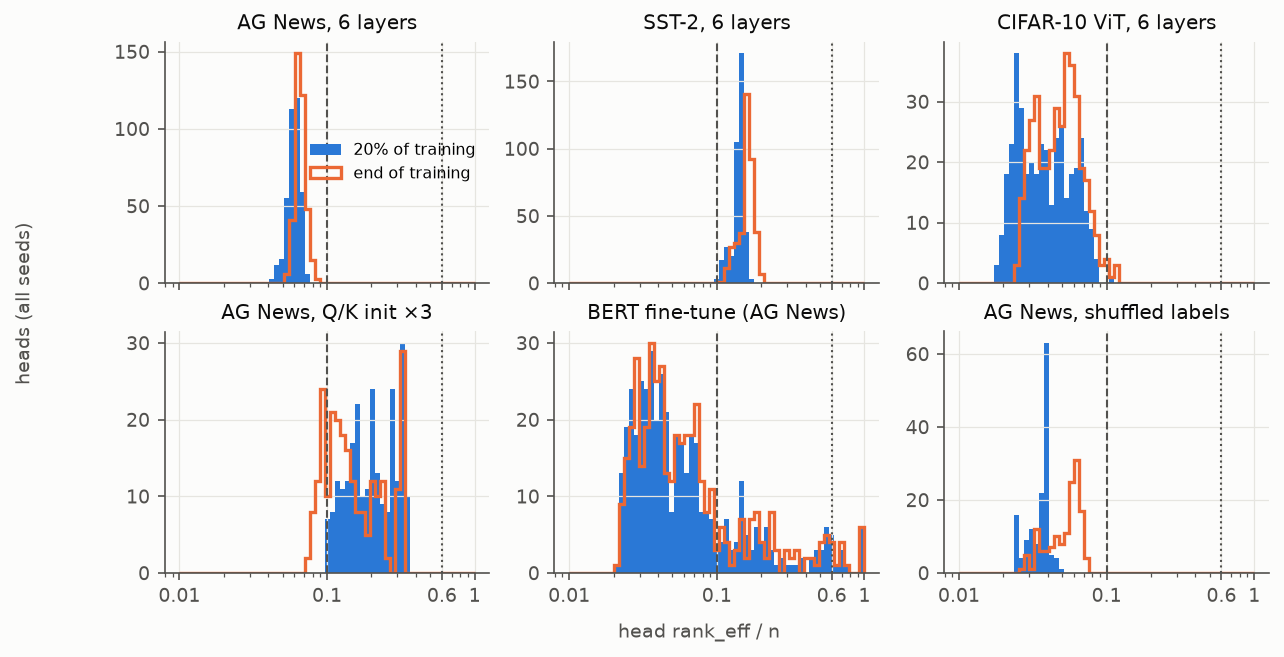
\includegraphics[width=0.95\linewidth]{figures/fig2_heads.png}
    \caption{Distribution of head $\reff/n$ at 20\% of training and at the end, over all seeds. Dashed and dotted lines mark the claimed limits of 0.1 and 0.6. Heads do not form two groups on either side of these limits; the only heads above 0.6 are in pretrained \bert.}
    \label{fig:heads}
\end{figure}

\begin{table}[t]
    \centering
    \small
    \begin{tabular}{@{}lrrrrr@{}}
        \toprule
        \textbf{Configuration} & \textbf{Share $>0.6n$} & \textbf{Share $<0.1n$} & \textbf{Between} & \textbf{Median $\reff/n$} & \textbf{Mean dip $p$} \\
        \midrule
        \cfg{ag\_L6} & 0.000 & 1.000 & 0.000 & 0.060 & .63 \\
        \cfg{sst\_L6} & 0.000 & 0.000 & 1.000 & 0.144 & .83 \\
        \cfg{cifar\_L6} & 0.000 & 0.997 & 0.003 & 0.036 & .74 \\
        \cfg{ag\_L6\_bigqk} & 0.000 & 0.012 & 0.988 & 0.200 & .35 \\
        \cfg{bert\_ag} & 0.030 & 0.778 & 0.192 & 0.047 & .99 \\
        \bottomrule
    \end{tabular}
    \caption{Head populations at 20\% of training, averaged over seeds. H1 needs at least 10\% of heads in both of the first two columns; no configuration comes close.}
    \label{tab:h1}
\end{table}

\begin{figure}[t]
    \centering
    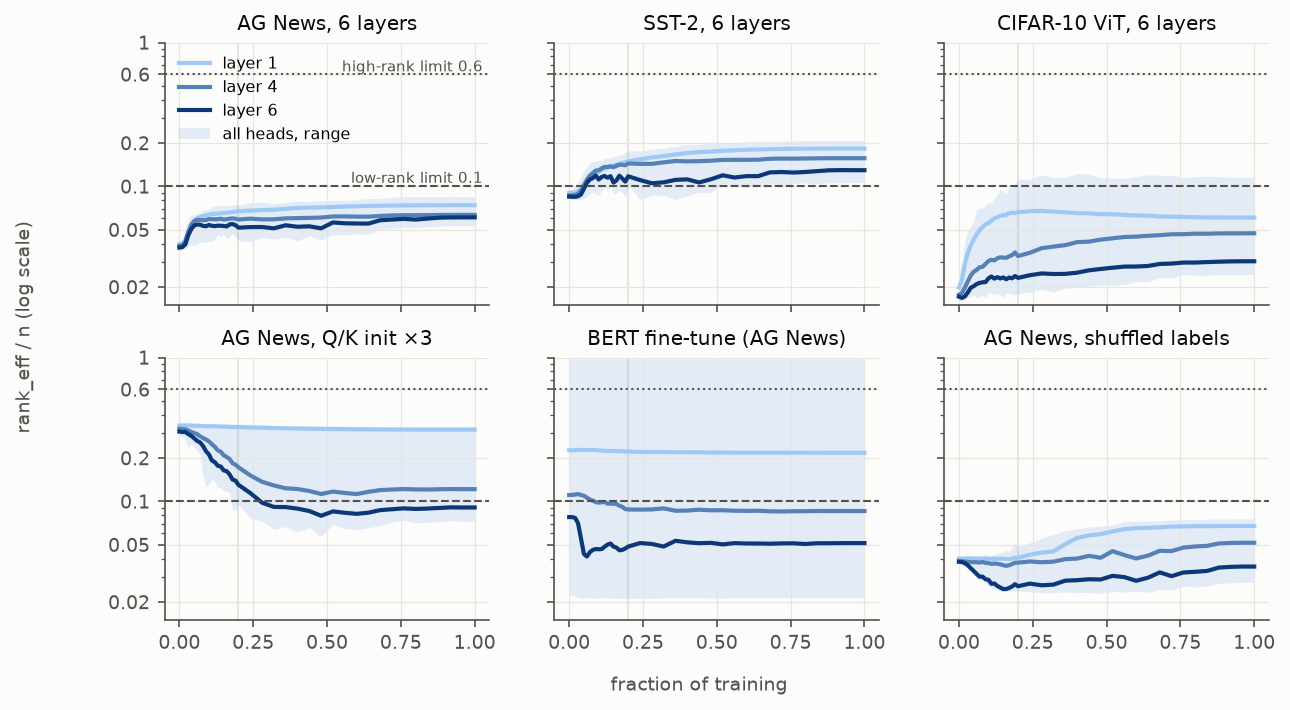
\includegraphics[width=0.95\linewidth]{figures/fig1_rank.png}
    \caption{$\reff/n$ over training on a log scale. Thick lines show first, middle, and last layers (seed means), and the band shows the range over all heads and seeds. Rank rises under default initialization (top row). Later layers lose rank from a peaked start (bottom left) and in pretrained \bert, while first layers keep their initial level. Without label signal (bottom right), the last layer dips and then recovers.}
    \label{fig:rank}
\end{figure}

\subsection{H2: entropy rises under default initialization}
\label{sec:h2}

{\bf The hypothesized pairing of an early monotone fall with a late U-shape occurs in no configuration} (\tabref{tab:h2}, \figref{fig:entropy}). In default arms, no early layer shows a monotone fall, and at most 5\% of late layers show a U-shape. Instead, entropy rises fast. The share of the total rank increase that occurs in the first 10\% of training is 77--86\% on \agnews (all depths and post-LN), 52--60\% on \sst and on \cifar at 3 and 6 layers, and 45\% on \cifar at 12 layers.

A late U-shape does appear in three settings: \cfg{cifar\_L6\_bigqk} (100\% of late layers), \cfg{ag\_L6\_shuffled} (100\%, 3 seeds), and \bert (67\%). It is not tied to large initialization alone, since \cfg{ag\_L6\_bigqk} shows a late fall with no rebound. Rather than a depth law, the U-shape looks like a transient that follows early over-concentration. Early \cifar layers show the opposite of a U: entropy peaks near 40\% of training and then declines slightly.

\begin{table}[t]
    \centering
    \small
    \begin{tabular}{@{}lcccccc@{}}
        \toprule
         & \multicolumn{2}{c}{$S/\log n$, start $\to$ end} & \multicolumn{2}{c}{Early layers} & Late layers \\
        \cmidrule(lr){2-3} \cmidrule(lr){4-5}
        \textbf{Configuration} & \textbf{Early layers} & \textbf{Late layers} & \textbf{Mono.\ fall} & \textbf{Mono.\ rise} & \textbf{U-shape} \\
        \midrule
        \cfg{ag\_L6} & .145 $\to$ .296 & .134 $\to$ .263 & 0\% & 94\% & 0\% \\
        \cfg{sst\_L6} & .159 $\to$ .394 & .143 $\to$ .316 & 0\% & 100\% & 0\% \\
        \cfg{cifar\_L6} & .053 $\to$ .331 & .027 $\to$ .172 & 0\% & 50\% & 0\% \\
        \cfg{ag\_L12} & .142 $\to$ .274 & .118 $\to$ .256 & 0\% & 35\% & 5\% \\
        \cfg{ag\_L6\_bigqk} & .708 $\to$ .636 & .686 $\to$ .353 & 50\% & 0\% & 0\% \\
        \cfg{cifar\_L6\_bigqk} & .367 $\to$ .419 & .322 $\to$ .213 & 0\% & 10\% & 100\% \\
        \cfg{ag\_L6\_shuffled} & .146 $\to$ .273 & .136 $\to$ .136 & 0\% & 50\% & 100\% \\
        \cfg{bert\_ag} & .428 $\to$ .428 & .184 $\to$ .204 & 0\% & 17\% & 67\% \\
        \bottomrule
    \end{tabular}
    \caption{Entropy shapes. Percentages are shares of (seed, layer) cells in the given band of layers. H2 needs a monotone fall early and a U-shape late in the same configuration.}
    \label{tab:h2}
\end{table}

\begin{figure}[t]
    \centering
    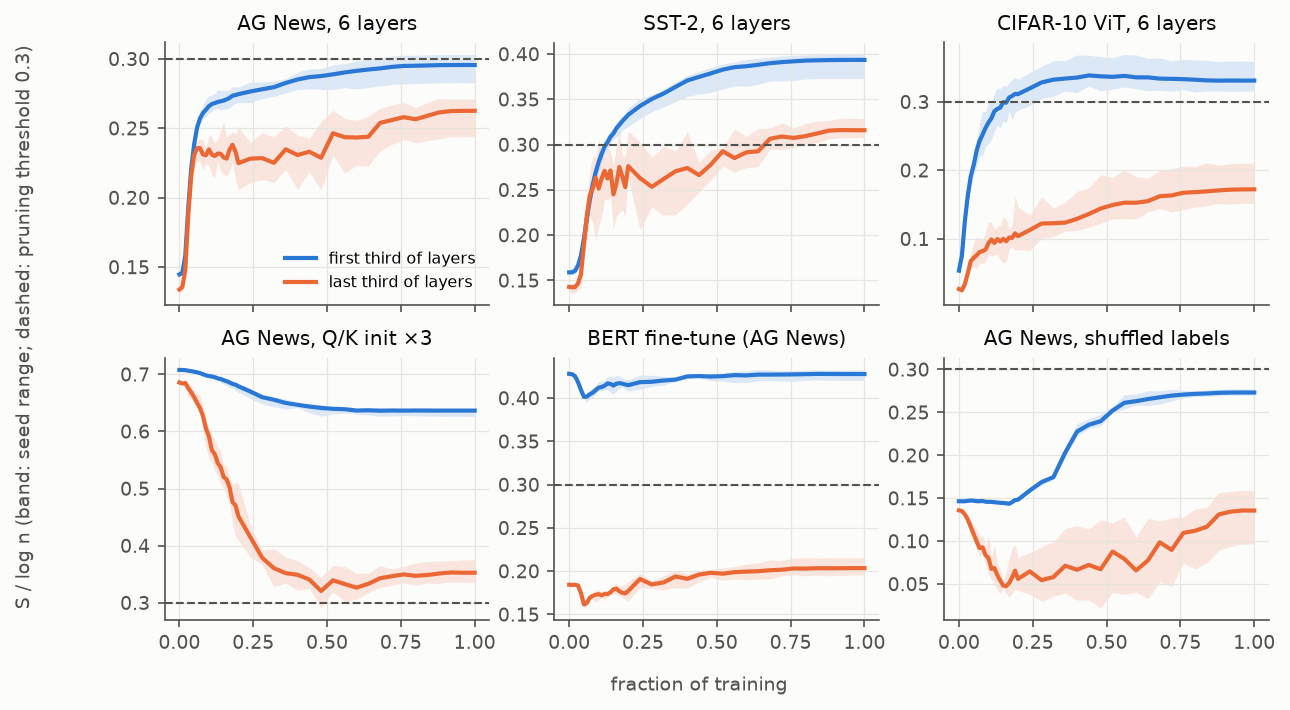
\includegraphics[width=0.95\linewidth]{figures/fig3_entropy.png}
    \caption{$S/\log n$ for the first and last thirds of layers; bands show the seed range and the dashed line marks the 0.3 pruning threshold. Default runs (top row) rise steeply and end near the threshold, which explains why it splits them so poorly (\secref{sec:h3}).}
    \label{fig:entropy}
\end{figure}

\subsection{H3: the threshold is not a safe pruning rule}
\label{sec:h3}

{\bf The rule passes in only 1 of 11 configurations with label signal} (\tabref{tab:h3}). Across \agnews and \cifar default arms it removes 63--96\% of heads at a cost of 19--45\pp. The reason is simple: attention is near-uniform, so most heads lie below $0.3\log n$, and the threshold selects most of the model instead of a redundant minority. \cfg{ag\_L6\_bigqk} has a small loss but prunes only 3.8\% of heads, which fails our non-vacuity rule.

\begin{table}[t]
    \centering
    \small
    \resizebox{\textwidth}{!}{%
    \begin{tabular}{@{}lrrrrrr@{}}
        \toprule
        \textbf{Configuration} & \textbf{Pruned} & \textbf{Low-$S$ loss [95\% CI]} & \textbf{Random} & \textbf{High-$S$} & \textbf{Oracle} & \textbf{Holm $p$ ($<2$\pp)} \\
        \midrule
        \cfg{sst\_L6} & 13.8\% & {\bf 0.12} [$-$0.43, 0.75] & 0.47 & 1.03 & 0.55 & .004 \\
        \cfg{ag\_L6\_bigqk} (vacuous) & 3.8\% & {\bf 0.12} [0.01, 0.27] & 0.24 & 0.22 & 0.26 & $<$.001 \\
        \cfg{ag\_L3} & 95.8\% & 45.3 [42.4, 48.2] & 42.1 & {\bf 39.2} & 43.3 & 1 \\
        \cfg{ag\_L6} & 84.9\% & 19.3 [16.4, 22.0] & {\bf 17.9} & 18.4 & 19.0 & 1 \\
        \cfg{ag\_L12} & 90.2\% & 24.1 [15.9, 31.6] & 25.8 & {\bf 23.7} & 24.2 & 1 \\
        \cfg{ag\_L6\_postln} & 89.2\% & 28.6 [20.4, 39.7] & 26.2 & 30.0 & {\bf 25.1} & 1 \\
        \cfg{cifar\_L3} & 63.3\% & 36.7 [28.2, 44.8] & 40.0 & 47.0 & {\bf 36.6} & 1 \\
        \cfg{cifar\_L6} & 66.9\% & {\bf 32.8} [28.8, 37.1] & 41.3 & 56.5 & 35.6 & 1 \\
        \cfg{cifar\_L12} & 70.0\% & {\bf 27.6} [23.8, 32.2] & 40.3 & 58.5 & 32.5 & 1 \\
        \cfg{cifar\_L6\_bigqk} & 46.7\% & 19.5 [17.5, 21.4] & 22.6 & 46.4 & {\bf 16.2} & 1 \\
        \cfg{bert\_ag} & 64.4\% & 40.9 [15.3, 58.6] & 13.6 & 25.5 & {\bf 7.6} & 1 \\
        \bottomrule
    \end{tabular}}
    \caption{Accuracy loss in percentage points at $\tau=0.3$, with all baselines at the same head count. The lowest loss in each row is in \textbf{bold}. Only \cfg{sst\_L6} passes with a non-vacuous cut. Shuffled-label runs are omitted.}
    \label{tab:h3}
\end{table}

\begin{figure}[t]
    \centering
    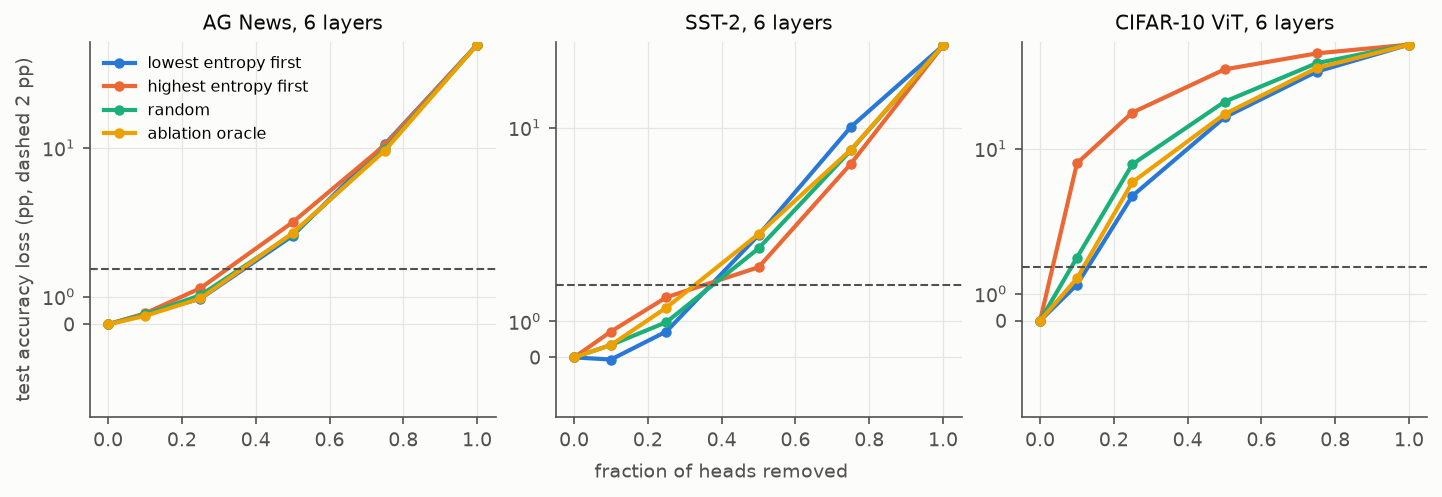
\includegraphics[width=0.95\linewidth]{figures/fig4_prune.png}
    \caption{Accuracy loss against share of heads removed for six-layer models, on a symmetric-log axis; the dashed line marks 2\pp. On \cifar, removing high-entropy heads first is far worse than the other rules, while on \agnews all rules coincide.}
    \label{fig:prune}
\end{figure}

\para{\sst.} The loss meets the criterion, but entropy adds nothing here: the difference from random is $-0.36$\pp (Wilcoxon $p=.25$). With 436 test sentences, one sentence is 0.23\pp, so this comparison is weak. \sst's normalized entropy ends higher than \agnews's (.32--.39 against .26--.30), so few heads fall below the line. Its sequences are also about half as long (mean $n$ of 22 against 46), and we did not test whether length is the cause.

\para{Entropy is a real signal on \cifar but not on text.} At the threshold's head count, removing low-entropy heads first beats random on all three default \cifar depths: by 8.5\pp at $L=6$ (Wilcoxon $p=.008$), 12.7\pp at $L=12$ ($t$-test $p=.005$), and 3.2\pp at $L=3$ ($t$-test $p=.002$). Removing high-entropy heads first costs far more, 56.5\pp against 32.8\pp at $L=6$. The Spearman correlation of $S$ with ablation importance is $+0.23$ to $+0.40$ on \cifar and $-0.14$ to $+0.11$ on default-initialization text. On \agnews, low-$S$ pruning is if anything worse than random, by 1.4\pp at $L=6$ (Wilcoxon $p=.016$). On \bert it is worse by 27\pp, though imprecisely (3 seeds, $t$-test $p=.12$). The ablation oracle does not always win, because single-head importance is a poor guide to joint removal.

\para{Smaller cuts and fine-tuning.} When we cut only 25\% of heads, default \agnews models and \sst lose 0.7--1.7\pp under every selection rule. This echoes \citet{michel2019sixteen}: much head removal is cheap under any method. \cifar at $L=6$ is different, losing 4.6\pp with low-$S$ first and 19.8\pp with high-$S$ first. Fine-tuning recovers much of the loss but not enough: \agnews goes from 19.3 to 10.4\pp and \cifar from 32.8 to 8.5\pp, while \sst stays at 0.12\pp.

\subsection{H4: the bound is false}
\label{sec:h4}

\begin{proposition}[Counterexample]
\label{prop:counter}
Let $X$ be uniform on $M\ge2$ inputs and $Y=f(X)$, so $H(Y|X)=0$. Take any network that computes $f$ and has a head whose attention map $x\mapsto\mA(x)$ is injective on these inputs, with that head's output weight set to zero. Predictions are unaffected, and since $\mA$ is a function of $X$, $I(\mA;X)=H(\mA)=\log M$ for every $n$. The right side of the claim tends to 0.
\end{proposition}

The training-set size cannot rescue the claim: $I(\mA;X)$ is a property of the map, and nothing forces a Bayes-optimal network's attention to discard input information. The direction is also suspect. The data-processing inequality gives $I(\mA;Y)\le I(X;Y)=H(Y)-H(Y|X)$, which falls with $H(Y|X)$, whereas the claim rises with it.

\begin{proposition}[Variance bound]
\label{prop:variance}
For $T=\mA(X)+\epsilon Z$ with $Z$ standard Gaussian and $\bar\mA=\E\,\mA(X)$,
\begin{equation*}
I(T;X)\le\min\Big\{\log M,\ \frac{\E\|\mA(X)-\bar\mA\|_F^2}{2\epsilon^2}\Big\}.
\end{equation*}
\end{proposition}
\begin{proof}
$I(T;X)=\E\,\mathrm{KL}(\gN(\mA(X),\epsilon^2I)\,\|\,P_T)\le\E\,\mathrm{KL}(\gN(\mA(X),\epsilon^2I)\,\|\,\gN(\bar\mA,\epsilon^2I))$, because the true marginal $P_T$ minimizes the expected KL over all reference distributions. The right side equals the variance term. The $\log M$ term follows from $I(T;X)\le H(X)$.
\end{proof}

What bounds the information is attention variability relative to the noise, and $H(Y|X)$ does not appear. $\Ibd$ stayed below this bound in all 19,200 checks (every layer, noise scale, and checkpoint). $\Ikl$ may exceed it, since Jensen's inequality only gives $\Ikl\le2\times$ the bound, and it does so at $\epsilon=2$.

\para{Measurements.} \Tabref{tab:h4} and \figref{fig:mi} show noise-free results. At $H(Y|X)=0$ and 100\% accuracy on \order ($n=32{,}000$), layer-level information is at least 1.04 nats on average, where the claim allows only $C/179$. Seeds vary widely here, from 0.21 to 1.83 nats. The per-head mean is 0.13 nats.

{\bf The excess does not shrink with $n$.} A true $O(1/\sqrt n)$ term needs a bounded $C$. On \agnews the implied $C$ rises from 7 to 180 at the layer level and from 0.9 to 23 at the head level. On \order it rises non-monotonically, from 40 to 186 and from 5 to 24. The \order trend is noisy and its $n=500$ cell did not learn the task, so \agnews carries more of the weight here. The regression also fails at every scale (\tabref{tab:regression}). Where the interval for $b$ includes 1 in the layer-level fits, the intercept is 1.4--5.5 nats, not near zero. On \agnews, $c$ is negative at every scale: information rises with $n$, the opposite of the claimed term.

{\bf Single numbers depend on the level and the noise scale.} At $\epsilon=2$, layer-level $\Ibd$ exceeds $H(Y|X)+1/\sqrt n$ in 93\% of \order runs and 73\% of \agnews runs. For the per-head mean these shares fall to 35\% and 15\%, and at $\epsilon=1$ they are 90\% and 47\%. Large noise can make the claim pass trivially: at $\epsilon=4$, noise-free \order runs at $n=8{,}000$ reach 0.13 nats. Cells below the claimed value are mostly noisy ones, such as \agnews at $\eta=0.4$, $n=500$ (0.32 against 1.11 nats), and these are consistent with the claim only because information is low there, not because it tracks $H(Y|X)$. An untrained network already exceeds the claim at low noise (\agnews at $\epsilon=1$: $\Ibd=0.65$ nats at step 0). For these reasons we rest the refutation on Proposition~\ref{prop:counter} and on the trend in $n$, and not on any one number.

Label noise does raise information, which fits the claim in sign only: at $n=32{,}000$ on \agnews, $\Ibd$ goes from 1.0 to 2.7 nats as $\eta$ goes from 0 to 0.4. Memorization of noisy labels is a likely mechanism, though we did not test it. Saturation is partial. At $n=8{,}000$, \agnews plateaus by 40\% of training and noise-free \order by 20\%, while \order at $\eta=0.2$ keeps rising (0.5 nats at 20\%, 3.8 at 60\%, 4.4 at the end). Plateaus do not sit at $H(Y|X)$.

\begin{figure}[t]
    \centering
    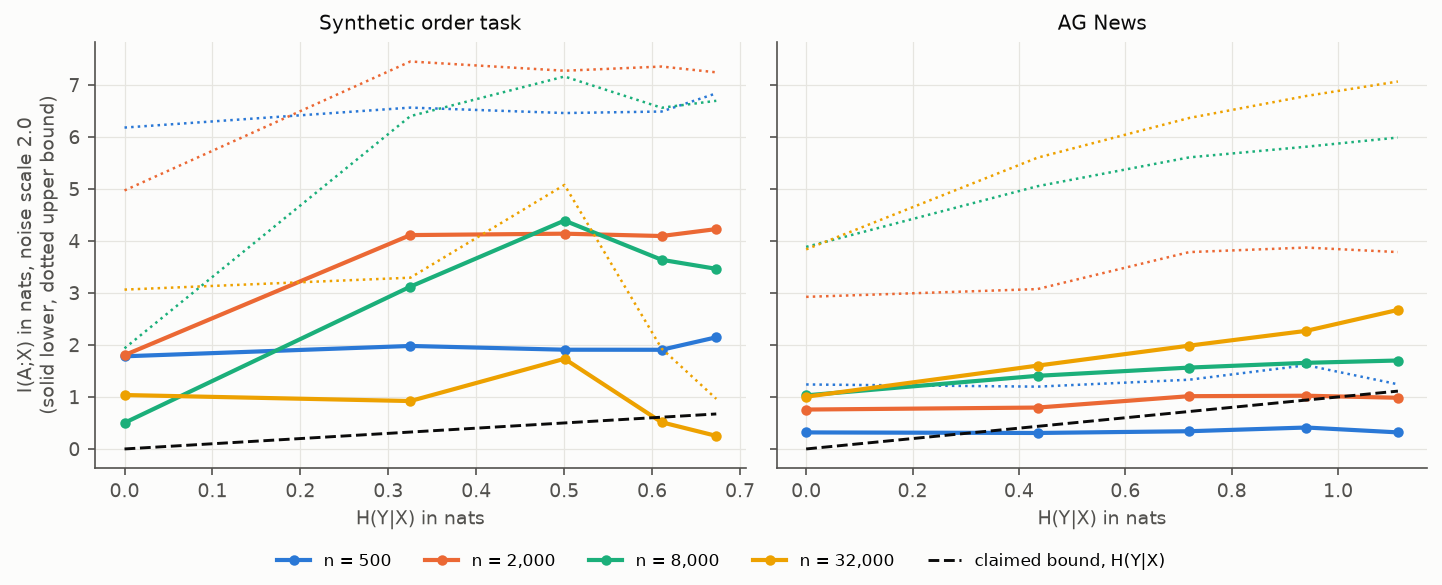
\includegraphics[width=0.95\linewidth]{figures/fig5_mi.png}
    \caption{Estimated layer-level information at $\epsilon=2$, averaged over layers and seeds. Solid lines are the lower bound and dotted lines the upper bound. The dashed black line is the claimed $H(Y|X)$ with the $O(1/\sqrt n)$ term set to zero. Noise-free points (left end) lie above the line at every $n$, and the curves do not approach it as $n$ grows.}
    \label{fig:mi}
\end{figure}

\begin{table}[t]
    \centering
    \small
    \begin{tabular}{@{}lrrrr@{}}
        \toprule
        \textbf{Noise-free runs, $\epsilon=2$} & \textbf{$n=500$} & \textbf{$n=2{,}000$} & \textbf{$n=8{,}000$} & \textbf{$n=32{,}000$} \\
        \midrule
        \order: layer $\Ibd$, nats (test accuracy) & 1.78 (49\%) & 1.80 (99\%) & 0.50 (100\%) & 1.04 (100\%) \\
        \order: implied $C$, layer / head & 40 / 5 & 81 / 10 & 45 / 6 & 186 / 24 \\
        \midrule
        \agnews: layer $\Ibd$, nats (test accuracy) & 0.32 (63\%) & 0.76 (76\%) & 1.03 (83\%) & 1.01 (87\%) \\
        \agnews: implied $C$, layer / head & 7 / 0.9 & 34 / 4 & 92 / 12 & 180 / 23 \\
        \bottomrule
    \end{tabular}
    \caption{Noise-free information. Implied $C$ is the excess of $\Ibd$ over $H(Y|X)$ times $\sqrt n$, which a true $O(1/\sqrt n)$ term would keep bounded. ``Layer'' treats all 8 heads jointly; ``head'' is the mean over heads.}
    \label{tab:h4}
\end{table}

\subsection{H5: depth shapes the size of the fall more than its speed}
\label{sec:h5}

\begin{table}[t]
    \centering
    \small
    \resizebox{\textwidth}{!}{%
    \begin{tabular}{@{}lccccl@{}}
        \toprule
        \textbf{Configuration} & \textbf{$t_{\min}$ layer 1} & \textbf{$t_{\min}$ last} & \textbf{Ratio [95\% CI]} & \textbf{Rank drop, first $\to$ last} & \textbf{Reading} \\
        \midrule
        \cfg{ag\_L3}, \cfg{ag\_L6}, \cfg{cifar\_L3} & 0 & 0 & undefined & 0 (rank rises) & Minimum at initialization \\
        \cfg{ag\_L12}, \cfg{cifar\_L6}, \cfg{cifar\_L12}, \cfg{sst\_L6} & $\le$.001 & .010--.124 & $\approx$0 & $\approx$0 & Same \\
        \cfg{ag\_L6\_bigqk} & .69 & .38 & {\bf 1.81} [1.63, 2.00] & 7\% $\to$ 75\% & Real collapse, below $3\times$ \\
        \cfg{cifar\_L6\_bigqk} & .002 & .14 & 0.01 [0, .04] & 0.4\% $\to$ 60\% & Layer 1 never falls \\
        \cfg{bert\_ag} & .63 & .05 & 11.9 [10.0, 14.4] & 4\% $\to$ 47\% & Layer 1 barely falls; unstable \\
        \bottomrule
    \end{tabular}}
    \caption{Time to minimum rank as a fraction of training. The criterion needs a fall of at least 10\% in both layers. No run in any configuration satisfies this.}
    \label{tab:h5}
\end{table}

{\bf Under default initialization there is no collapse to time} (\tabref{tab:h5}). The minimum sits at or near the start, because rank rises: $\reff/n$ goes from .04 to .07 on \agnews (layer 1), .09 to .18 on \sst, and .02 to .06 on \cifar. Three signal configurations show a real fall in deep layers. \cfg{ag\_L6\_bigqk} gives the only interpretable ratio, 1.81, which is below the claimed range, and even there layer 1 falls only 7\%. In \cfg{cifar\_L6\_bigqk} and \bert, layer 1 hardly falls, so the ratio has little meaning. Without label signal, the last layer of \cfg{ag\_L6\_shuffled} drops 37\% and then recovers, so a transient fall does not need a peaked start.

Post-hoc rise times to peak rank have no consistent sign (\figref{fig:depth}). The mean per-seed ratios of layer 1 to last layer are 7.8, 2.1, and 0.63 on \agnews for $L=3,6,12$, and 0.42, 0.26, and 0.21 on \cifar. The value of 2.1 hides heavy tails: its median is 0.78. \sst gives 3.7 [2.4, 5.0], which overlaps the claimed range, but this measures a different quantity on a post-hoc basis.

{\bf What holds up is the size of the fall.} From a peaked start, the rank drop grows steadily with depth: 7, 36, 56, 66, 70, and 75\% from layer 1 to 6 on \agnews, and 0.4, 14, 30, 42, 53, and 60\% on \cifar. \bert's 4\% to 47\% matches this pattern. In addition, the first layer has higher rank than the last at 95--100\% of checkpoints in every configuration, though not always in strict order across intermediate layers. This agrees with \citet{wang2020linformer}, who report more skewed spectra in higher layers.

\begin{figure}[t]
    \centering
    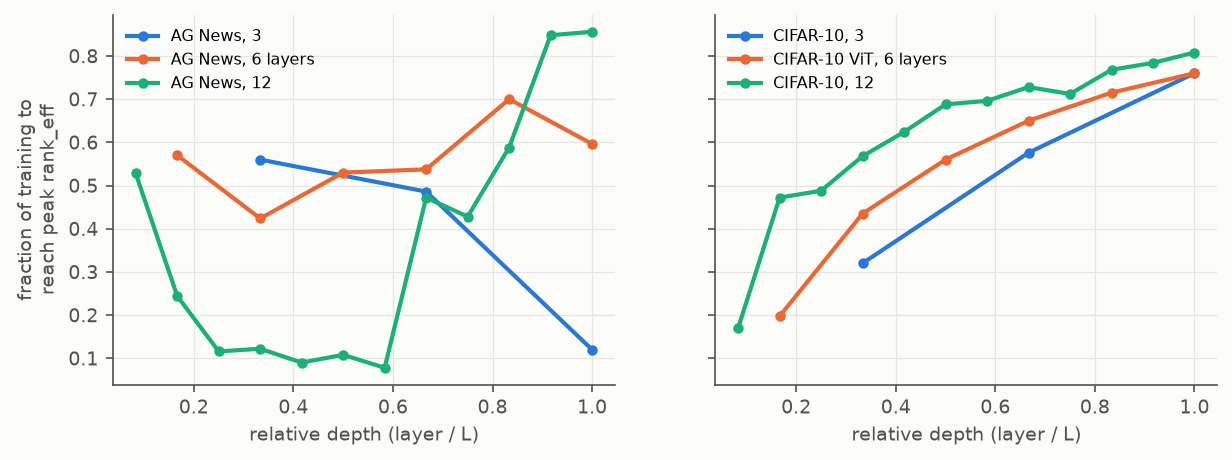
\includegraphics[width=0.8\linewidth]{figures/fig6_depth.png}
    \caption{Fraction of training needed for $\reff$ to reach its peak, by relative depth and network size, under default initialization. \cifar peaks later in deeper layers, while \agnews shows no consistent order. The direction of the depth effect depends on the task.}
    \label{fig:depth}
\end{figure}

\section{Discussion}
\label{sec:discussion}

\para{Why did the framing fail?} The hypothesis imagines full-rank matrices that collapse. With standard initialization, scaled dot-product attention begins near-uniform (row entropy about 0.99) because queries and keys are small, so $\mA$ is close to a rank-one matrix and learning builds structure. The $\times3$ arm is the key control. When attention starts peaked (row entropy 0.48, $\reff/n$ about 0.32 on \agnews), rank falls, and falls more with depth. Last layers then end close together from either side, at .06 for default and .09 for $\times3$ on \agnews, though first layers keep their starting level (.07 and .32). The start state therefore persists early in the network and matters less late in it. \bert starts peaked as well (row entropy about 0.50), and its last layers lose rank during fine-tuning, which agrees with this reading.

\para{Practical implications.} We advise against a fixed $0.3\log n$ cut-off for pruning. Descriptions of attention training as rank collapse should state the initial state, since it sets the direction. On vision models, entropy is a useful ranking signal, but this does not carry over to text. We did not expect this split. One possible reason is that a fixed image grid gives heads stable spatial roles while text attention varies by input, but we did not test this.

\para{Alternative explanations.} {\it Small models:} \bert is far larger and pretrained, and it is also unimodal and mostly low-rank (mean dip $p=.99$). {\it Pre-LN:} post-LN matched pre-LN almost exactly. {\it \textsc{cls} pooling:} this was constant across arms, so we cannot rule out an effect. {\it Averaging across inputs:} per-head means could hide bimodality at the level of single inputs, and this is a real limitation.

\para{Limitations.} We study small encoders and short fine-tunes on three classification datasets. We did not study ImageNet-scale vision transformers, decoders, or large language models, where bifurcation might hold, although nothing here suggests it. The definitions of $\reff$ and $S$ were our choice, as the hypothesis gave none, and five rank definitions cover only H1. The $\times3$ arm, rise-time ratios, $\epsilon=2$ as reporting scale, and paired baseline tests were not pre-registered, and we tested only one gain value, so these analyses are exploratory.

For H3, \sst evaluation has 436 sentences, \bert has 3 seeds with very wide intervals, and we ran fine-tuning only on $L=6$ default arms. Zeroing a head without rescaling is one of several removal methods.

For H4, noise channels define a quantity only relative to $\epsilon$. Layer-level and per-head values differ by about a factor of eight at a fixed $\epsilon\ge1$, and the claim does not say which it means. \agnews's intrinsic $H(Y|X)$ is assumed near zero and is really some small unknown value. Injected noise applies to training labels, while clean test inputs supply $X$. On \order, training failed at small $n$ (test accuracy near 50\% at $n=500$ and for noisy runs at $n=2{,}000$), and 3-seed means are noisy. Our reading of $n$ as training-set size is an assumption. A derivation with stronger assumptions, such as stochastic attention or a different left side such as $I(\mA;Y)$, could survive, but it would not be this claim.

Time to minimum uses a 5\% tolerance on 41 checkpoints, so differences below about 1\% of training early on, or 4\% later, cannot be resolved. Shared-GPU restarts should not affect results, and the exact rerun supports this, but it covered one configuration on one GPU type.

\section{Conclusion}
\label{sec:conclusion}

We tested five claims about attention spectra over training, with per-head tracking across 68 runs and 120 information runs. Heads do not split into high- and low-rank populations. Under standard initialization they start near-uniform and gain rank, so rank collapse is not a universal training dynamic. The bound $I(A;X)\le H(Y|X)+O(1/\sqrt n)$ is false, and our variance bound is a valid replacement. The $0.3\log n$ pruning rule is unsafe, though entropy carries pruning information on \cifar. One finding survives in modified form: the rank fall from peaked starts grows strongly with depth.

{\bf The takeaway:} the initial state, not training alone, decides whether attention rank falls.

Future work should sweep query and key gain and softmax temperature to map how the start state carries through depth, test a per-layer entropy ranking on larger vision models, ask whether stable spatial roles explain the link between entropy and importance on vision, and analyze per-input distributions, since per-head means may hide input-level bimodality. If a derivation of the H4 bound exists, its assumptions deserve a direct test.


\bibliography{references}

\appendix
\section{Information Regressions at All Noise Scales}
\label{app:regression}

\begin{table}[h]
    \centering
    \small
    \begin{tabular}{@{}llrrrr@{}}
        \toprule
        \textbf{Task} & $\epsilon$ & \textbf{$a$ [95\% CI]} & \textbf{$b$ [95\% CI]} & \textbf{$c$} & \textbf{Mean $\Ibd$} \\
        \midrule
        \order & 0.5 & 5.33 [4.45, 6.20] & 0.79 [$-$0.74, 2.32] & 52.2 & 6.76 \\
         & 1 & 3.06 [1.94, 4.19] & 2.23 [0.25, 4.21] & 71.1 & 5.50 \\
         & 2 & 1.38 [0.71, 2.05] & 1.94 [0.70, 3.17] & 9.0 & 2.38 \\
         & 4 & 0.36 [0.18, 0.53] & 0.50 [0.18, 0.83] & 2.1 & 0.61 \\
        \midrule
        \agnews & 0.5 & 8.33 [8.01, 8.65] & 0.18 [$-$0.19, 0.56] & $-$75.4 & 6.87 \\
         & 1 & 5.54 [5.11, 5.97] & 1.47 [1.00, 1.95] & $-$118.4 & 4.00 \\
         & 2 & 1.58 [1.43, 1.74] & 0.59 [0.35, 0.82] & $-$38.3 & 1.16 \\
         & 4 & 0.40 [0.36, 0.44] & 0.15 [0.09, 0.22] & $-$9.9 & 0.30 \\
        \bottomrule
    \end{tabular}
    \caption{Layer-level fits of $\Ibd=a+bH(Y|X)+c/\sqrt n$. The $\epsilon=0.2$ fits are omitted since they sit at the $\log M$ ceiling, and $\epsilon\le1$ is ceiling-affected. No scale gives both $b$ near 1 and $a$ near 0. Per-head fits at $\epsilon=2$ give $a=0.18$, $b=0.25$ [0.09, 0.41] on \order and $a=0.20$, $b=0.08$ [0.05, 0.11] on \agnews, so they also fail.}
    \label{tab:regression}
\end{table}

\section{Deviations from the Plan}
\label{app:deviations}

The plan was frozen before training. We changed the following afterwards: (1) the noise grid moved from $\{.05$--$1\}$ to $\{.2$--$4\}$ after a pilot showed that small scales pin at the ceiling; (2) we added the $\times3$ arm after the first 5 runs; (3) we gathered the literature by hand; (4) we added the correlation of $S$ with ablation importance as a descriptive statistic; (5) fine-tuning moved to a separate script that uses saved weights, so it was not available for \bert; (6) the job queue was reordered and GPU reservations lowered for the information and \bert runs; (7) we chose $\epsilon=2$ after seeing the data; (8) we added rise-time ratios because time to minimum is degenerate under default initialization. All planned seeds finished.


\end{document}
